% Options for packages loaded elsewhere
\PassOptionsToPackage{unicode}{hyperref}
\PassOptionsToPackage{hyphens}{url}
%
\documentclass[
]{book}
\usepackage{lmodern}
\usepackage{amssymb,amsmath}
\usepackage{ifxetex,ifluatex}
\ifnum 0\ifxetex 1\fi\ifluatex 1\fi=0 % if pdftex
  \usepackage[T1]{fontenc}
  \usepackage[utf8]{inputenc}
  \usepackage{textcomp} % provide euro and other symbols
\else % if luatex or xetex
  \usepackage{unicode-math}
  \defaultfontfeatures{Scale=MatchLowercase}
  \defaultfontfeatures[\rmfamily]{Ligatures=TeX,Scale=1}
\fi
% Use upquote if available, for straight quotes in verbatim environments
\IfFileExists{upquote.sty}{\usepackage{upquote}}{}
\IfFileExists{microtype.sty}{% use microtype if available
  \usepackage[]{microtype}
  \UseMicrotypeSet[protrusion]{basicmath} % disable protrusion for tt fonts
}{}
\makeatletter
\@ifundefined{KOMAClassName}{% if non-KOMA class
  \IfFileExists{parskip.sty}{%
    \usepackage{parskip}
  }{% else
    \setlength{\parindent}{0pt}
    \setlength{\parskip}{6pt plus 2pt minus 1pt}}
}{% if KOMA class
  \KOMAoptions{parskip=half}}
\makeatother
\usepackage{xcolor}
\IfFileExists{xurl.sty}{\usepackage{xurl}}{} % add URL line breaks if available
\IfFileExists{bookmark.sty}{\usepackage{bookmark}}{\usepackage{hyperref}}
\hypersetup{
  pdftitle={Estadística I: Análisis exploratorio de datos y muestreo},
  pdfauthor={Rodrigo Zepeda-Tello},
  hidelinks,
  pdfcreator={LaTeX via pandoc}}
\urlstyle{same} % disable monospaced font for URLs
\usepackage{color}
\usepackage{fancyvrb}
\newcommand{\VerbBar}{|}
\newcommand{\VERB}{\Verb[commandchars=\\\{\}]}
\DefineVerbatimEnvironment{Highlighting}{Verbatim}{commandchars=\\\{\}}
% Add ',fontsize=\small' for more characters per line
\usepackage{framed}
\definecolor{shadecolor}{RGB}{248,248,248}
\newenvironment{Shaded}{\begin{snugshade}}{\end{snugshade}}
\newcommand{\AlertTok}[1]{\textcolor[rgb]{0.94,0.16,0.16}{#1}}
\newcommand{\AnnotationTok}[1]{\textcolor[rgb]{0.56,0.35,0.01}{\textbf{\textit{#1}}}}
\newcommand{\AttributeTok}[1]{\textcolor[rgb]{0.77,0.63,0.00}{#1}}
\newcommand{\BaseNTok}[1]{\textcolor[rgb]{0.00,0.00,0.81}{#1}}
\newcommand{\BuiltInTok}[1]{#1}
\newcommand{\CharTok}[1]{\textcolor[rgb]{0.31,0.60,0.02}{#1}}
\newcommand{\CommentTok}[1]{\textcolor[rgb]{0.56,0.35,0.01}{\textit{#1}}}
\newcommand{\CommentVarTok}[1]{\textcolor[rgb]{0.56,0.35,0.01}{\textbf{\textit{#1}}}}
\newcommand{\ConstantTok}[1]{\textcolor[rgb]{0.00,0.00,0.00}{#1}}
\newcommand{\ControlFlowTok}[1]{\textcolor[rgb]{0.13,0.29,0.53}{\textbf{#1}}}
\newcommand{\DataTypeTok}[1]{\textcolor[rgb]{0.13,0.29,0.53}{#1}}
\newcommand{\DecValTok}[1]{\textcolor[rgb]{0.00,0.00,0.81}{#1}}
\newcommand{\DocumentationTok}[1]{\textcolor[rgb]{0.56,0.35,0.01}{\textbf{\textit{#1}}}}
\newcommand{\ErrorTok}[1]{\textcolor[rgb]{0.64,0.00,0.00}{\textbf{#1}}}
\newcommand{\ExtensionTok}[1]{#1}
\newcommand{\FloatTok}[1]{\textcolor[rgb]{0.00,0.00,0.81}{#1}}
\newcommand{\FunctionTok}[1]{\textcolor[rgb]{0.00,0.00,0.00}{#1}}
\newcommand{\ImportTok}[1]{#1}
\newcommand{\InformationTok}[1]{\textcolor[rgb]{0.56,0.35,0.01}{\textbf{\textit{#1}}}}
\newcommand{\KeywordTok}[1]{\textcolor[rgb]{0.13,0.29,0.53}{\textbf{#1}}}
\newcommand{\NormalTok}[1]{#1}
\newcommand{\OperatorTok}[1]{\textcolor[rgb]{0.81,0.36,0.00}{\textbf{#1}}}
\newcommand{\OtherTok}[1]{\textcolor[rgb]{0.56,0.35,0.01}{#1}}
\newcommand{\PreprocessorTok}[1]{\textcolor[rgb]{0.56,0.35,0.01}{\textit{#1}}}
\newcommand{\RegionMarkerTok}[1]{#1}
\newcommand{\SpecialCharTok}[1]{\textcolor[rgb]{0.00,0.00,0.00}{#1}}
\newcommand{\SpecialStringTok}[1]{\textcolor[rgb]{0.31,0.60,0.02}{#1}}
\newcommand{\StringTok}[1]{\textcolor[rgb]{0.31,0.60,0.02}{#1}}
\newcommand{\VariableTok}[1]{\textcolor[rgb]{0.00,0.00,0.00}{#1}}
\newcommand{\VerbatimStringTok}[1]{\textcolor[rgb]{0.31,0.60,0.02}{#1}}
\newcommand{\WarningTok}[1]{\textcolor[rgb]{0.56,0.35,0.01}{\textbf{\textit{#1}}}}
\usepackage{longtable,booktabs}
% Correct order of tables after \paragraph or \subparagraph
\usepackage{etoolbox}
\makeatletter
\patchcmd\longtable{\par}{\if@noskipsec\mbox{}\fi\par}{}{}
\makeatother
% Allow footnotes in longtable head/foot
\IfFileExists{footnotehyper.sty}{\usepackage{footnotehyper}}{\usepackage{footnote}}
\makesavenoteenv{longtable}
\usepackage{graphicx,grffile}
\makeatletter
\def\maxwidth{\ifdim\Gin@nat@width>\linewidth\linewidth\else\Gin@nat@width\fi}
\def\maxheight{\ifdim\Gin@nat@height>\textheight\textheight\else\Gin@nat@height\fi}
\makeatother
% Scale images if necessary, so that they will not overflow the page
% margins by default, and it is still possible to overwrite the defaults
% using explicit options in \includegraphics[width, height, ...]{}
\setkeys{Gin}{width=\maxwidth,height=\maxheight,keepaspectratio}
% Set default figure placement to htbp
\makeatletter
\def\fps@figure{htbp}
\makeatother
\setlength{\emergencystretch}{3em} % prevent overfull lines
\providecommand{\tightlist}{%
  \setlength{\itemsep}{0pt}\setlength{\parskip}{0pt}}
\setcounter{secnumdepth}{5}
\usepackage{booktabs}
\usepackage[]{natbib}
\bibliographystyle{apalike}

\title{Estadística I: Análisis exploratorio de datos y muestreo}
\author{Rodrigo Zepeda-Tello}
\date{2020-08-05}

\begin{document}
\maketitle

{
\setcounter{tocdepth}{1}
\tableofcontents
}
\hypertarget{prefacio}{%
\chapter{Prefacio}\label{prefacio}}

Hola

\hypertarget{intro}{%
\chapter{Introduction}\label{intro}}

You can label chapter and section titles using \texttt{\{\#label\}} after them, e.g., we can reference Chapter \ref{intro}. If you do not manually label them, there will be automatic labels anyway, e.g., Chapter \ref{methods}.

Figures and tables with captions will be placed in \texttt{figure} and \texttt{table} environments, respectively.

\begin{Shaded}
\begin{Highlighting}[]
\KeywordTok{par}\NormalTok{(}\DataTypeTok{mar =} \KeywordTok{c}\NormalTok{(}\DecValTok{4}\NormalTok{, }\DecValTok{4}\NormalTok{, }\FloatTok{.1}\NormalTok{, }\FloatTok{.1}\NormalTok{))}
\KeywordTok{plot}\NormalTok{(pressure, }\DataTypeTok{type =} \StringTok{'b'}\NormalTok{, }\DataTypeTok{pch =} \DecValTok{19}\NormalTok{)}
\end{Highlighting}
\end{Shaded}

\begin{figure}

{\centering 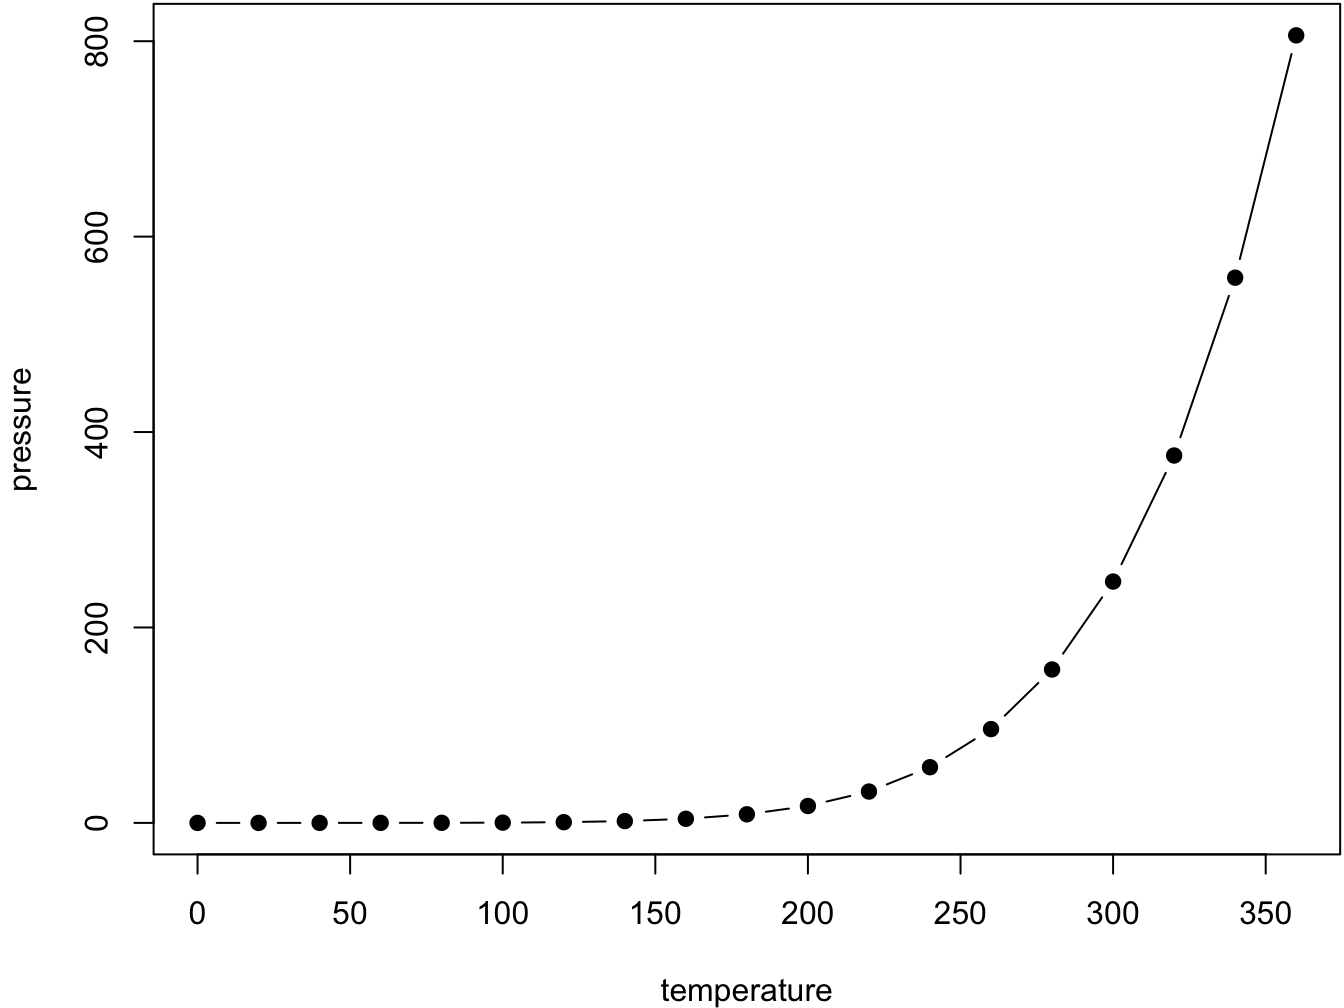
\includegraphics[width=0.8\linewidth]{Introduccion_a_Muestreo_files/figure-latex/nice-fig-1} 

}

\caption{Here is a nice figure!}\label{fig:nice-fig}
\end{figure}

Reference a figure by its code chunk label with the \texttt{fig:} prefix, e.g., see Figure \ref{fig:nice-fig}. Similarly, you can reference tables generated from \texttt{knitr::kable()}, e.g., see Table \ref{tab:nice-tab}.

\begin{Shaded}
\begin{Highlighting}[]
\NormalTok{knitr}\OperatorTok{::}\KeywordTok{kable}\NormalTok{(}
  \KeywordTok{head}\NormalTok{(iris, }\DecValTok{20}\NormalTok{), }\DataTypeTok{caption =} \StringTok{'Here is a nice table!'}\NormalTok{,}
  \DataTypeTok{booktabs =} \OtherTok{TRUE}
\NormalTok{)}
\end{Highlighting}
\end{Shaded}

\begin{table}

\caption{\label{tab:nice-tab}Here is a nice table!}
\centering
\begin{tabular}[t]{rrrrl}
\toprule
Sepal.Length & Sepal.Width & Petal.Length & Petal.Width & Species\\
\midrule
5.1 & 3.5 & 1.4 & 0.2 & setosa\\
4.9 & 3.0 & 1.4 & 0.2 & setosa\\
4.7 & 3.2 & 1.3 & 0.2 & setosa\\
4.6 & 3.1 & 1.5 & 0.2 & setosa\\
5.0 & 3.6 & 1.4 & 0.2 & setosa\\
\addlinespace
5.4 & 3.9 & 1.7 & 0.4 & setosa\\
4.6 & 3.4 & 1.4 & 0.3 & setosa\\
5.0 & 3.4 & 1.5 & 0.2 & setosa\\
4.4 & 2.9 & 1.4 & 0.2 & setosa\\
4.9 & 3.1 & 1.5 & 0.1 & setosa\\
\addlinespace
5.4 & 3.7 & 1.5 & 0.2 & setosa\\
4.8 & 3.4 & 1.6 & 0.2 & setosa\\
4.8 & 3.0 & 1.4 & 0.1 & setosa\\
4.3 & 3.0 & 1.1 & 0.1 & setosa\\
5.8 & 4.0 & 1.2 & 0.2 & setosa\\
\addlinespace
5.7 & 4.4 & 1.5 & 0.4 & setosa\\
5.4 & 3.9 & 1.3 & 0.4 & setosa\\
5.1 & 3.5 & 1.4 & 0.3 & setosa\\
5.7 & 3.8 & 1.7 & 0.3 & setosa\\
5.1 & 3.8 & 1.5 & 0.3 & setosa\\
\bottomrule
\end{tabular}
\end{table}

You can write citations, too. For example, we are using the \textbf{bookdown} package \citep{R-bookdown} in this sample book, which was built on top of R Markdown and \textbf{knitr} \citep{xie2015}.

\hypertarget{appendix-apuxe9ndice}{%
\appendix}


\hypertarget{programaciuxf3n-en-r}{%
\chapter{\texorpdfstring{Programación en \texttt{R}}{Programación en R}}\label{programaciuxf3n-en-r}}

\begin{figure}

{\centering 
\includegraphics[width=150px]{images/rlogo} 

}

\caption{`R` es un programa chido de estadística. FIN.}\label{fig:unnamed-chunk-3}
\end{figure}

Una de las primeras cosas que necesitamos saber es que \texttt{R} (por más que sus más ávidos defensores digan lo contrario) no es para todo. Si tú ya conoces otro lenguaje (sea \texttt{Stata}, \texttt{Excel}, \texttt{SAS}, \texttt{Python}, \texttt{Matlab}, \texttt{Julia}, etc) sabrás utilizar muchas de sus opciones. Estoy seguro que, de conocer uno de estos, te será muchísimo más fácil seguir sacando promedios en tu lenguaje favorito que en \texttt{R}, realizar regresiones lineales es probablemente más sencillo en \texttt{Stata} mientras que las gráficas de barras para mí son más simples en \texttt{Excel}, \texttt{Python} excede en aplicaciones de inteligencia artificial mientras que \texttt{Matlab} es más veloz que \texttt{R}, \texttt{Julia} tiene muchas cosas de ecuaciones diferenciales que nadie más.

Lo que probablemente no sea más sencillo de hacer en otro lenguaje es realizar análisis estadístico, gráficas de todo tipo y modelos de simulación. Para eso, \texttt{R} es, indiscutiblemente, una de las mejores opciones para quienes no conocen de programación\footnote{Modelos de simulación más avanzados suelen hacerse en \texttt{C}, \texttt{C++} o \texttt{Fortran} por su velocidad; empero, es necesario conocer más de programación.}.

Finalmente, uno de los consejos más importantes que te puedo dar es que este curso no te va a servir si no practicas. Igual que como pasa con los idiomas uno no aprende \texttt{R} en una semana \emph{sin practicarlo después}. Mi sugerencia es que, a la vez que sigues estas notas comiences a trabajar un proyecto \emph{tuyo} específico junto con \href{https://yandex.com}{el buscador de Internet de tu preferencia} a la mano y empieces a usar \texttt{R} en él. Practica\footnote{La práctica hace al maestro}.

\hypertarget{algunas-ventajas-de-r-y-cosas-no-tan-padres}{%
\section{\texorpdfstring{Algunas ventajas de \texttt{R} y cosas no tan padres}{Algunas ventajas de R y cosas no tan padres}}\label{algunas-ventajas-de-r-y-cosas-no-tan-padres}}

\hypertarget{puntos-a-favor-de-r}{%
\subsection{\texorpdfstring{Puntos a favor de \texttt{R}}{Puntos a favor de R}}\label{puntos-a-favor-de-r}}

\begin{itemize}
\item
  Todo el mundo lo usa. Quizá éste es el punto más a favor. Si mucha gente lo conoce y lo utiliza, hay más opciones de ayuda. Los sitios de StackOverflow \href{https://stackoverflow.com}{en inglés} y \href{https://es.stackoverflow.com}{en español} son excelentes para pedir apoyo en \texttt{R}; los \href{https://groups.google.com/forum/\#!forum/r-help-archive}{grupos de usuarios de Google} son otra fuente muy buena. Entre más gente usa el programa; es más fácil obtener ayuda porque seguro alguien más tuvo hace ya tiempo el mismo problema que tú.
\item
  Todas las personas que trabajan en estadística publican sus métodos y su código en \texttt{R} (eso, claro, cuando publican sus métodos). Es raro encontrar \emph{un nuevo método estadístico} en el mundo y que no se pueda usar, de alguna forma, en \texttt{R}.
\item
  Dentro de los lenguajes de programación \texttt{R} es de los más sencillos. Quienes lo hicieron realmente se preocuparon por su público (de no especialistas) y en general desarrollan para él.
\item
  \texttt{R} es gratis. Y en esta época de austeridad, cualquier ahorro es bueno. Que sea gratis no significa que no esté respaldado: existen versiones de \texttt{R} respaldadas por grandes compañías como \href{https://mran.microsoft.com/open}{Microsoft}
\item
  Todo lo que se hace en \texttt{R} es público. \texttt{R} no tiene métodos secretos ni es una caja negra. Todo lo que hace cada una de las funciones de \texttt{R}, cualquiera lo puede revisar, por completo.
\item
  En \texttt{R} puedes hacer libros o notas ¡como este! donde guardes todo tu trabajo, reportes automatizados e incluso \href{https://gallery.shinyapps.io/086-bus-dashboard/}{documentos interactivos} para facilitar el análisis de datos.
\item
  \texttt{R} puede hacer gráficas bonitas:
\end{itemize}

\begin{center}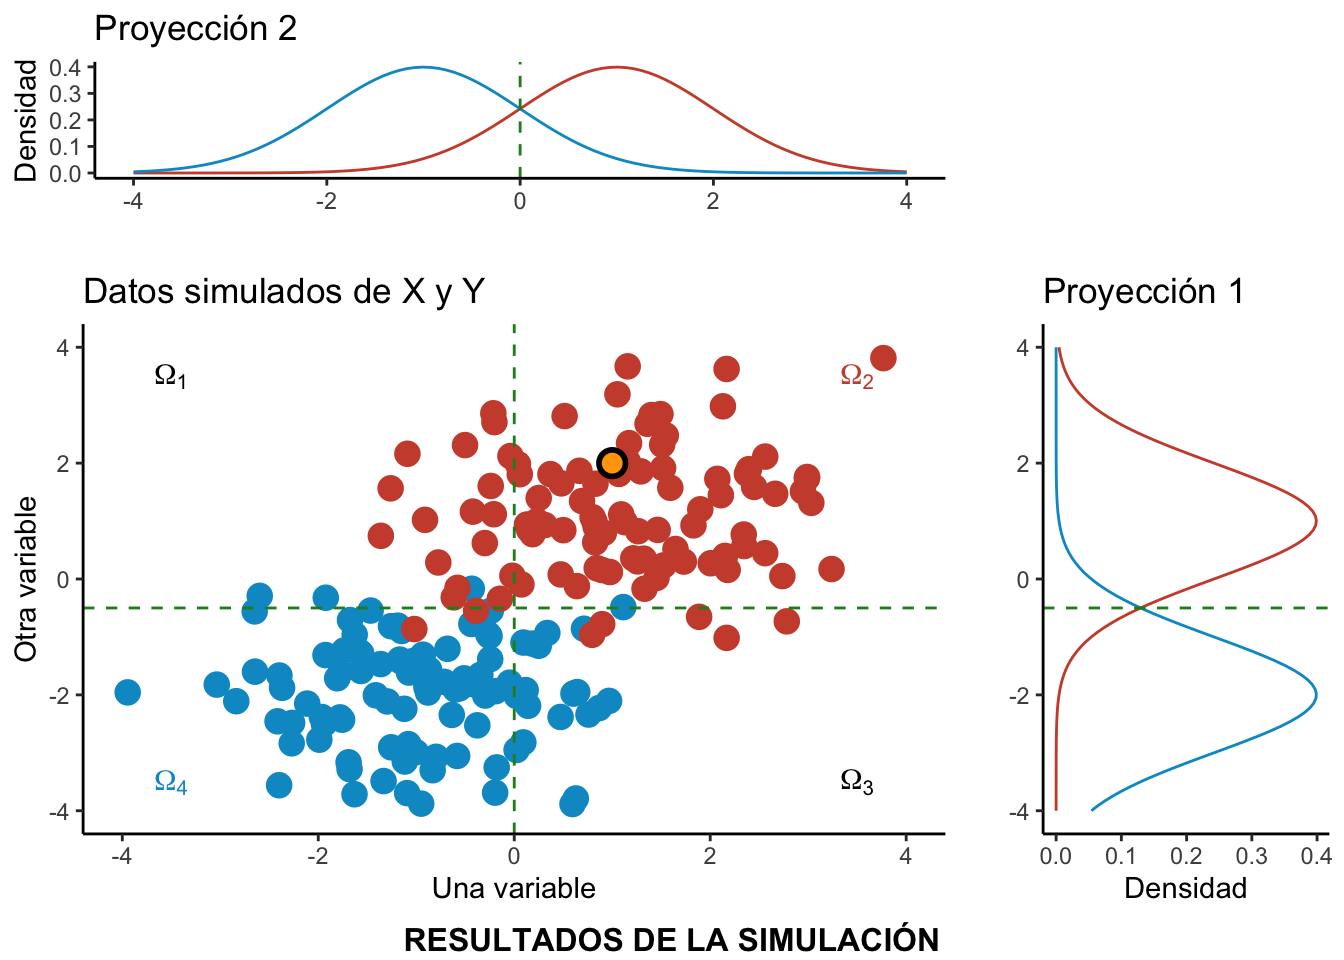
\includegraphics{Introduccion_a_Muestreo_files/figure-latex/unnamed-chunk-4-1} \end{center}

Por supuesto, no todo es miel sobre hojuelas con \texttt{R}. Particularmente, algunos de los problemas con el lenguaje:

\begin{figure}

{\centering 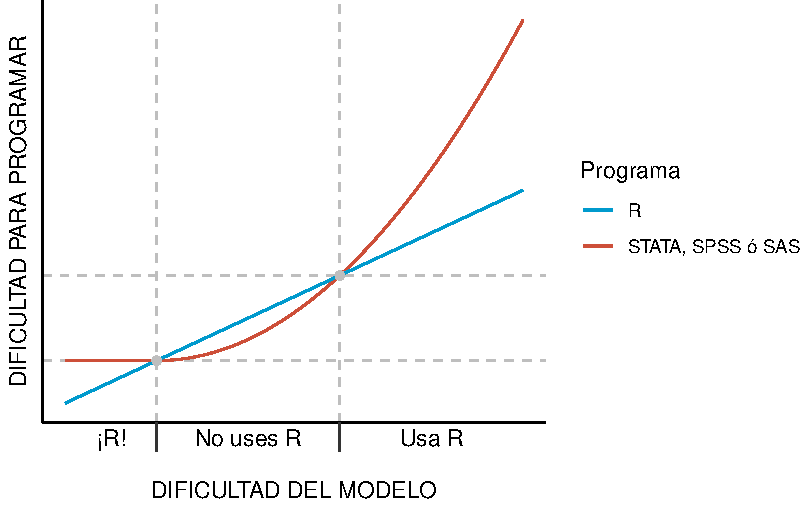
\includegraphics{Introduccion_a_Muestreo_files/figure-latex/unnamed-chunk-5-1} 

}

\caption{La curva de aprendizaje de `R` es más empinada pero después de un rato vale la pena}\label{fig:unnamed-chunk-5}
\end{figure}

\begin{itemize}
\item
  La curva de aprendizaje es mucho más empinada que para otros programas estadísticos (como \texttt{Stata}, \texttt{SAS} o \texttt{SPSS}) ¡particularmente si es tu primera vez programando!
\item
  La mayor parte de las personas que trabajan en \texttt{R} no son programadores de verdad. Gran parte del código que te puedes encontrar \textbf{en el mundo real} está escrito \href{https://nsaunders.wordpress.com/2014/05/14/this-is-why-code-written-by-scientists-gets-ugly/}{con prisa para salir del aprieto} sin mucha planeación, con pocos comentarios, falta de control de versiones y pocas herramientas de revisión. ¡Internet está lleno de \href{https://codegolf.stackexchange.com/a/4011}{creaturas espantosas escritas en \texttt{R}}!
\end{itemize}

\begin{figure}

{\centering 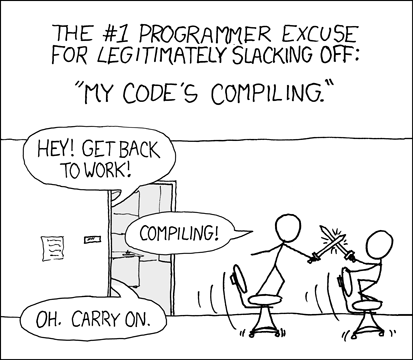
\includegraphics[width=5.74in]{images/compiling} 

}

\caption{`R` puede ser muy lento pero eso te da oportunidad de hacer otras cosas ;) .}\label{fig:unnamed-chunk-6}
\end{figure}

\begin{itemize}
\tightlist
\item
  \texttt{R} \href{https://github.com/matthieugomez/benchmark-stata-r}{de ninguna manera es veloz} por lo que algunos programas (lo veremos en simulación) pueden ser extremada (y dolorosamente) lentos.
\end{itemize}

\hypertarget{bienvenidx-a-r-taking-off-again-suxed-asuxed-se-llama-esta-versiuxf3n}{%
\section{\texorpdfstring{Bienvenidx a \texttt{R}, Taking Off Again (sí, así se llama esta versión)}{Bienvenidx a R, Taking Off Again (sí, así se llama esta versión)}}\label{bienvenidx-a-r-taking-off-again-suxed-asuxed-se-llama-esta-versiuxf3n}}

\texttt{R} es un lenguaje de cómputo y un programa estadístico \href{https://www.gnu.org/philosophy/free-sw.html}{libre}, gratuito, \href{http://adv-r.had.co.nz/Functional-programming.html}{de programación funcional} (¿qué es eso?), \href{https://en.wikipedia.org/wiki/Object-oriented_programming}{orientado a objetos} (\emph{what??}) que mutó a partir de otros dos lenguajes conocidos como \texttt{Scheme} y \texttt{S}\footnote{De ahí que se llame \texttt{R} porque la \texttt{R} es una mejor letra que la \texttt{S} (todos lo sabemos)
  -Atte. Rodrigo, el autor de este documento.}. El primero de estos fue desarrollado en el MIT por Sussman y Steele mientras que el segundo surgió en los laboratorios Bell\footnote{Mejor conocidos ahora como AT\&T, la compañía celular que nunca tiene señal.} creado por Becker, Wilks y Chambers. \texttt{R} \href{https://cran.r-project.org/doc/html/interface98-paper/paper_2.html}{nació en junio de 1995} a partir del trabajo de Ross Ihaka y Robert Gentleman\footnote{Sus nombres empiezan con la letra \texttt{R} ¿coincidencia?}.

Desde su creación, la mayor parte del desarrollo de \texttt{R} ha sido trabajo completamente voluntario de la \href{https://www.r-project.org/foundation/}{Fundación R}, del equipo de R Core y de miles de usuarios que han creado funciones específicas para \texttt{R} conocidas como paquetes (\texttt{packages}). Actualmente el repositorio más importante de \texttt{R}, CRAN, contiene más de \emph{16000} paquetes con distintas funciones para hacer ¡lo que quieras!

Como todo el trabajo en \texttt{R} es voluntario hace falta:

\begin{enumerate}
\def\labelenumi{\arabic{enumi}.}
\item
  Una homologación en los métodos. Puedes encontrar varias funciones \emph{que supuestamente hacen exactamente lo mismo} (como es el caso de \texttt{emojifont}, \texttt{fontemoji} y \texttt{emoGG} para graficar usando emojis).
\item
  Estandarizar la notación. Algunos paquetes como aquellos del \texttt{tidyverse} (veremos más adeltna) utilizan \texttt{pipes} (\texttt{\%\textgreater{}\%}); estos sólo funcionan en el \texttt{tidyverse} pero no fuera del mismo.
\end{enumerate}

Sin embargo, también es una gran ventaja que sean los usuarios de \texttt{R} quienes guían su desarrollo. El lenguaje va mutando según peticiones de las personas que lo usan. Si hay algo que te gustaría \texttt{R} tuviera y aún no existe ¡lo puedes proponer!

\hypertarget{instalando-cosas}{%
\section{Instalando cosas}\label{instalando-cosas}}

\hypertarget{instalaciuxf3n-de-r}{%
\subsection{\texorpdfstring{Instalación de \texttt{R}}{Instalación de R}}\label{instalaciuxf3n-de-r}}

\begin{figure}

{\centering 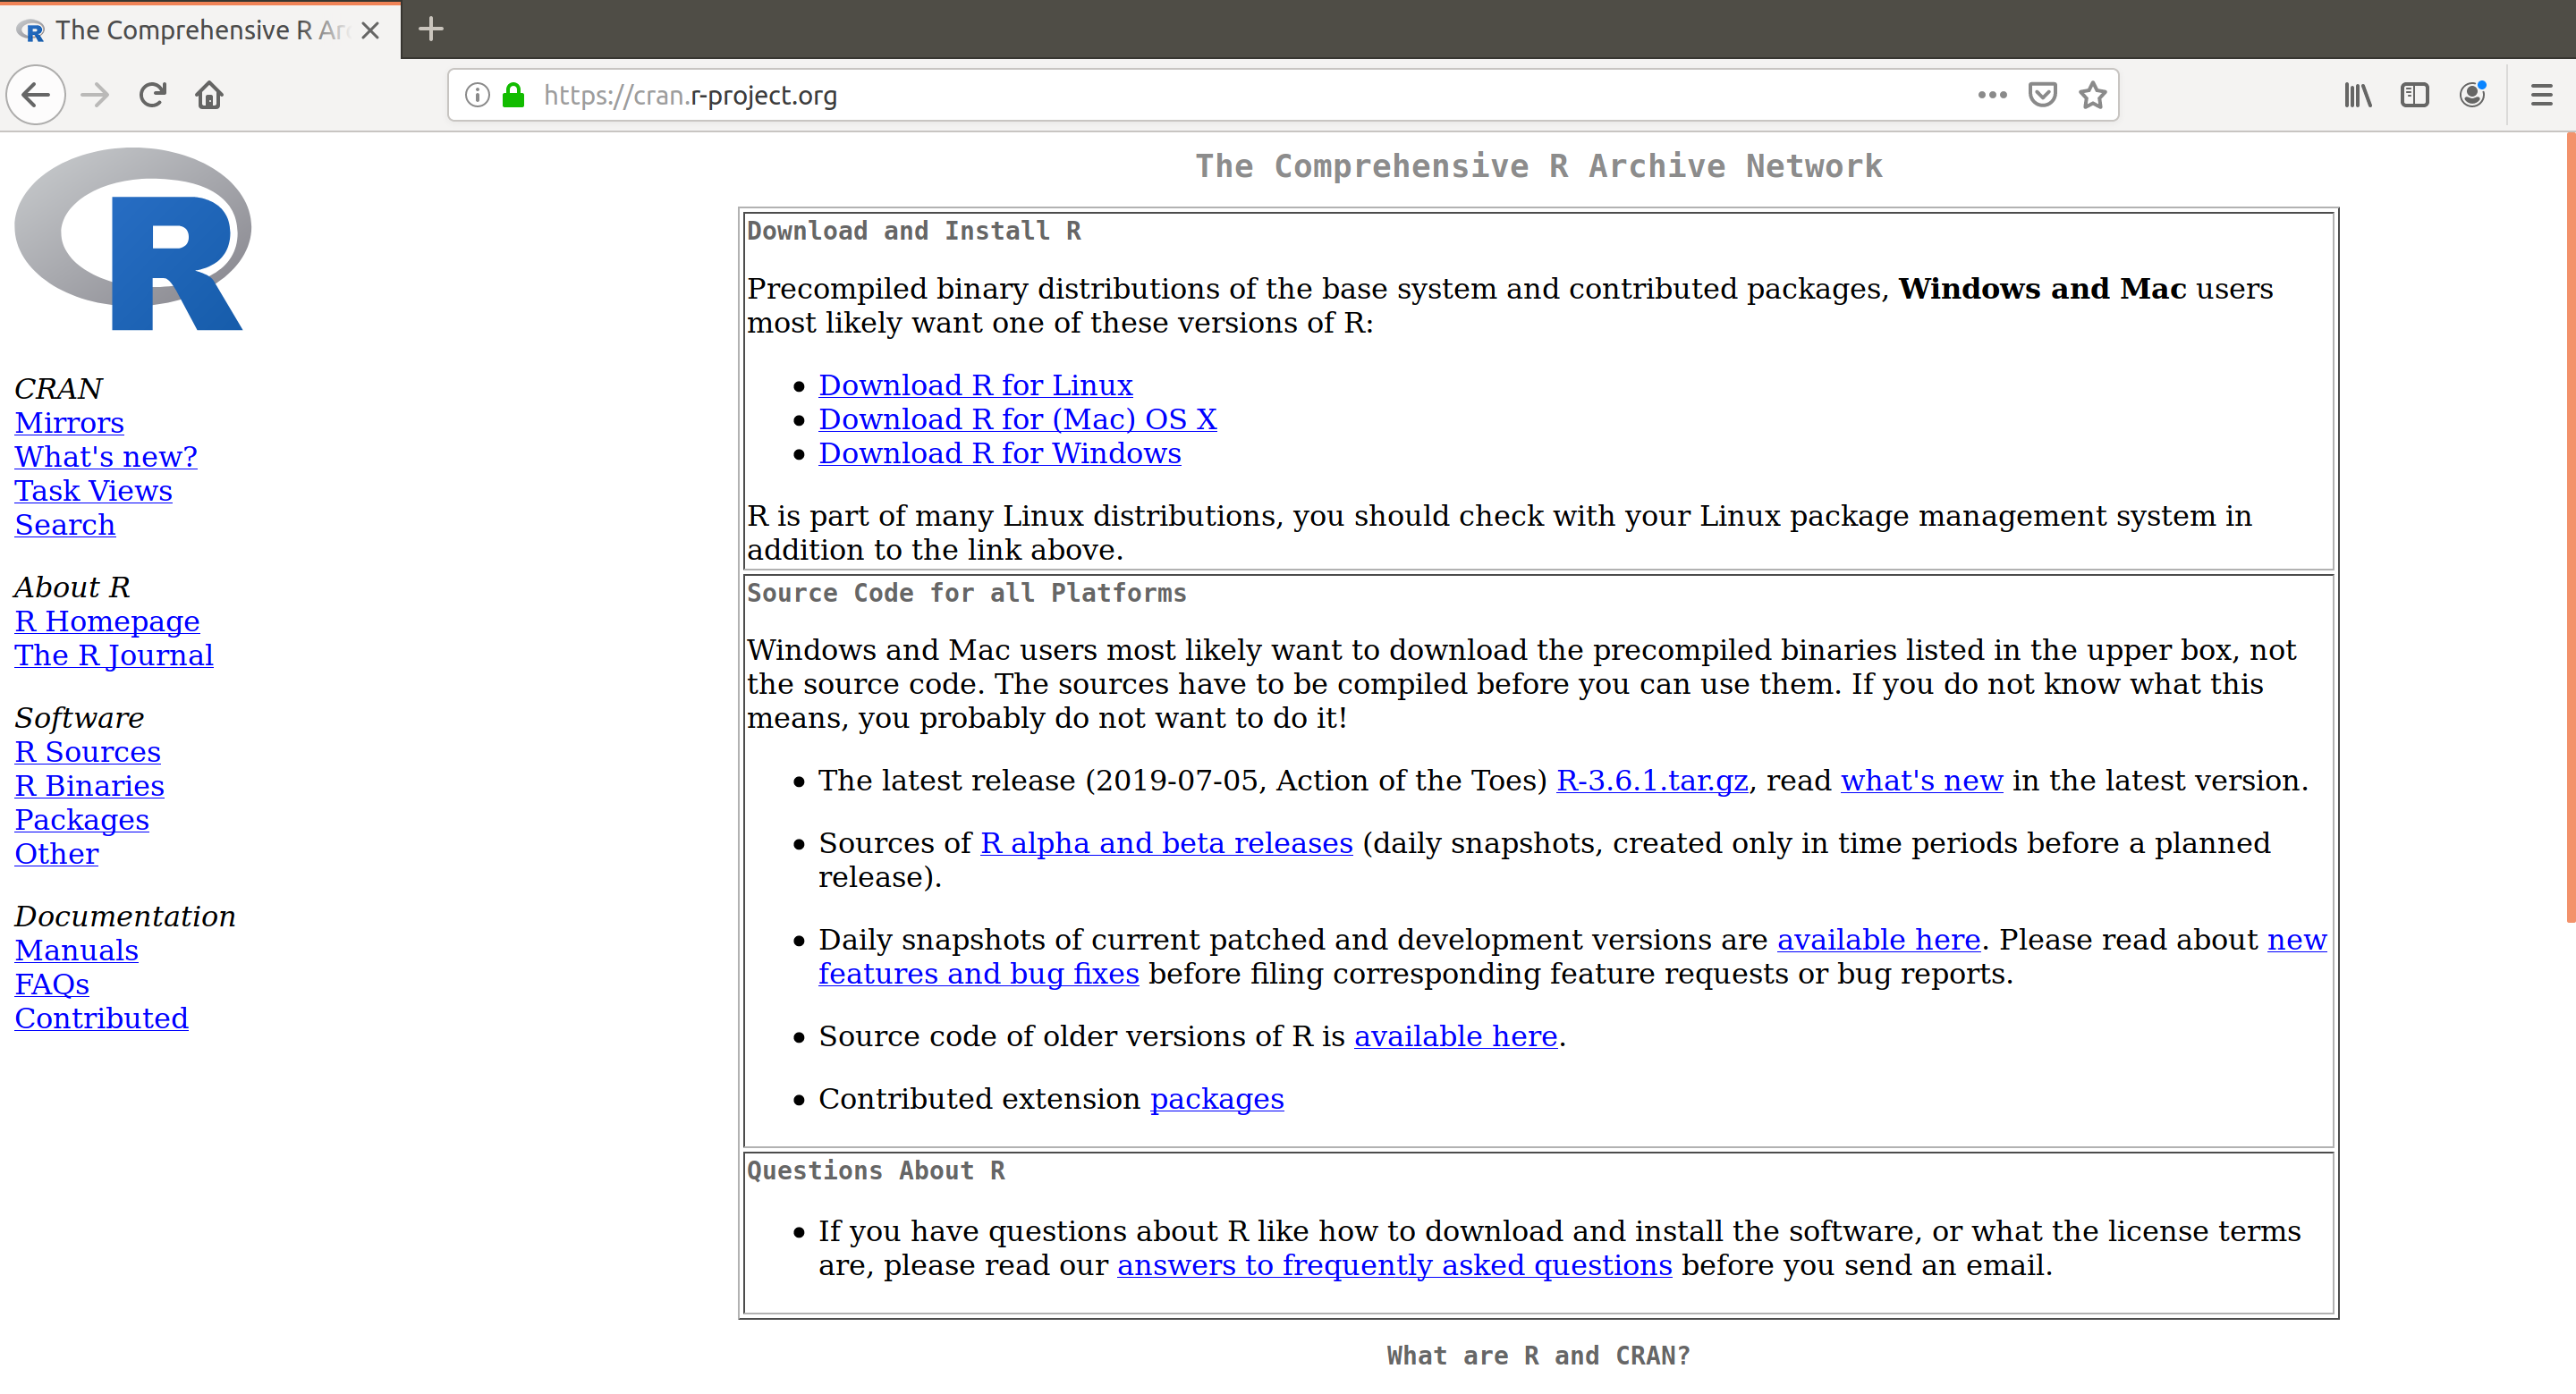
\includegraphics[width=40in]{images/CRAN1} 

}

\caption{Oficialmente, la página de `R` es de las páginas más feas del mundo. ¡No te dejes llevar por las apariencias!}\label{fig:unnamed-chunk-7}
\end{figure}

A lo largo de estas notas estaré trabajando con: R version 4.0.2 (2020-06-22) \emph{Taking Off Again}. La más reciente versión de \texttt{R} la puedes encontrar en \href{https://cran.r-project.org}{CRAN}. Para ello ve al sitio y selecciona tu plataforma.

\begin{quote}
\textbf{Nota usuarios de Mac} En algunas Mac, al abir R, aparece el siguiente mensaje de advertencia:
\texttt{During\ startup\ -\ Warning\ messages:\ 1:\ Setting\ LC\_CTYPE\ failed\ {[}...{]}}
para \href{https://stackoverflow.com/questions/9689104/installing-r-on-mac-warning-messages-setting-lc-ctype-failed-using-c}{solucionarlo} ve a \texttt{Aplicaciones} y abre \texttt{Terminal}. Copia y pega en ella el siguiente texto:
\texttt{defaults\ write\ org.R-project.R\ force.LANG\ en\_US.UTF-8}
Da enter, cierra la \texttt{Terminal} y reinicia \texttt{R}.
\end{quote}

\begin{itemize}
\tightlist
\item
  En el caso de Windows da clic en \texttt{Download\ R\ for\ Windows} y luego en \texttt{install\ R\ for\ the\ first\ time}. Finalmente, ejecuta el instalable que aparece al dar click en \texttt{Download\ R\ 4.0.2\ for\ Windows} .
\end{itemize}

\begin{quote}
Para este curso pudiera ser que requirieras las herramientas de desarrollador \href{https://cran.r-project.org/bin/windows/Rtools/}{Rtools}.
\end{quote}

\begin{itemize}
\item
  En el caso de Mac selecciona \texttt{Download\ R\ for\ (Mac)\ OS\ X} y luego elige \texttt{R-4.0.2.pkg}. En Mac puede que necesites instalar adicionalmente \href{https://www.xquartz.org}{XQuartz} (según tu versión de Mac). Si tu Mac es una versión suficientemente antigua, sigue las instrucciones específicas de \texttt{CRAN}.
\item
  En el caso de Linux al elegir \texttt{Download\ R\ for\ Linux} tendrás la opción de buscar tu distribución específica. Al elegirla, aparecerán instrucciones para tu terminal de comandos; síguelas. En el caso de Linux, según los paquetes de \texttt{R} que elijamos instalar en la computadora requerirás instalar paquetería adicional para tu distribución de Linux. \texttt{R} te informará de la paquetería necesaria conforme la requiera.
\end{itemize}

\begin{quote}
Si tienes problemas para instalar puedes usar \href{https://rstudio.cloud}{RStudio Cloud}.
\end{quote}

\hypertarget{instalaciuxf3n-de-rstudio}{%
\section{\texorpdfstring{Instalación de \texttt{RStudio}}{Instalación de RStudio}}\label{instalaciuxf3n-de-rstudio}}

\begin{figure}

{\centering 
\includegraphics[width=49.08in]{images/rstudio} 

}

\caption{RStudio es una empresa que se dedica a hacer cosas para R.}\label{fig:unnamed-chunk-8}
\end{figure}

\texttt{RStudio} es una interfaz gráfica (IDE) para \texttt{R}. Puedes pensar a \texttt{R} como el \emph{Bloc de Notas} y a \texttt{RStudio} como \emph{Word}. El \emph{Bloc} tiene todas las capacidades que necesitas para poder escribir; empero, es muchísimo mejor trabajar tus \emph{papers} en \emph{Word}. De la misma manera, \texttt{R} tiene todas las capacidades para hacer estadística \emph{pero un formato horrible} y \texttt{RStudio} se ha convertido en la más popular forma de usar \texttt{R}. Por supuesto que no es la única; algunas alternativas son \href{https://atom.io/packages/ide-r}{Atom con ide-r}, \href{https://marketplace.eclipse.org/content/statet-r}{Eclipse con StatET} y \href{https://rkward.kde.org}{RKWard}. En general es posible seguir estas notas sin que tengas \texttt{RStudio} pero, si es tu primera vez programando, no lo recomiendo.

\begin{quote}
Si ya tienes experiencia con lenguajes como Python, Javascript, Java ó alguno de los mil C que existen, no tendrás ningún problema usando el editor de tu preferencia.
\end{quote}

Para descargar \texttt{RStudio} ve a \href{https://www.rstudio.com}{su página} y da clic en \texttt{Download\ RStudio}. Baja tu pantalla hasta donde dice \texttt{Installers\ for\ Supported\ Platforms} y elige tu plataforma: \texttt{Windows}, \texttt{Mac\ OS\ X} ó tu sabor de \texttt{Linux} preferido. Una vez descargado el archivo, ábrelo y sigue las instrucciones que aparecen en pantalla.

\hypertarget{primeros-pasos-en-r-usando-rstudio}{%
\section{\texorpdfstring{Primeros pasos en \texttt{R} usando \texttt{RStudio}}{Primeros pasos en R usando RStudio}}\label{primeros-pasos-en-r-usando-rstudio}}

Una vez hayas instalado \texttt{R} y \texttt{RStudio}, abre \texttt{RStudio}\footnote{Si decidiste no instalar RStudio salta al final de esta sección.}. Te enfrentarás a una pantalla similar a esta:

\begin{figure}

{\centering 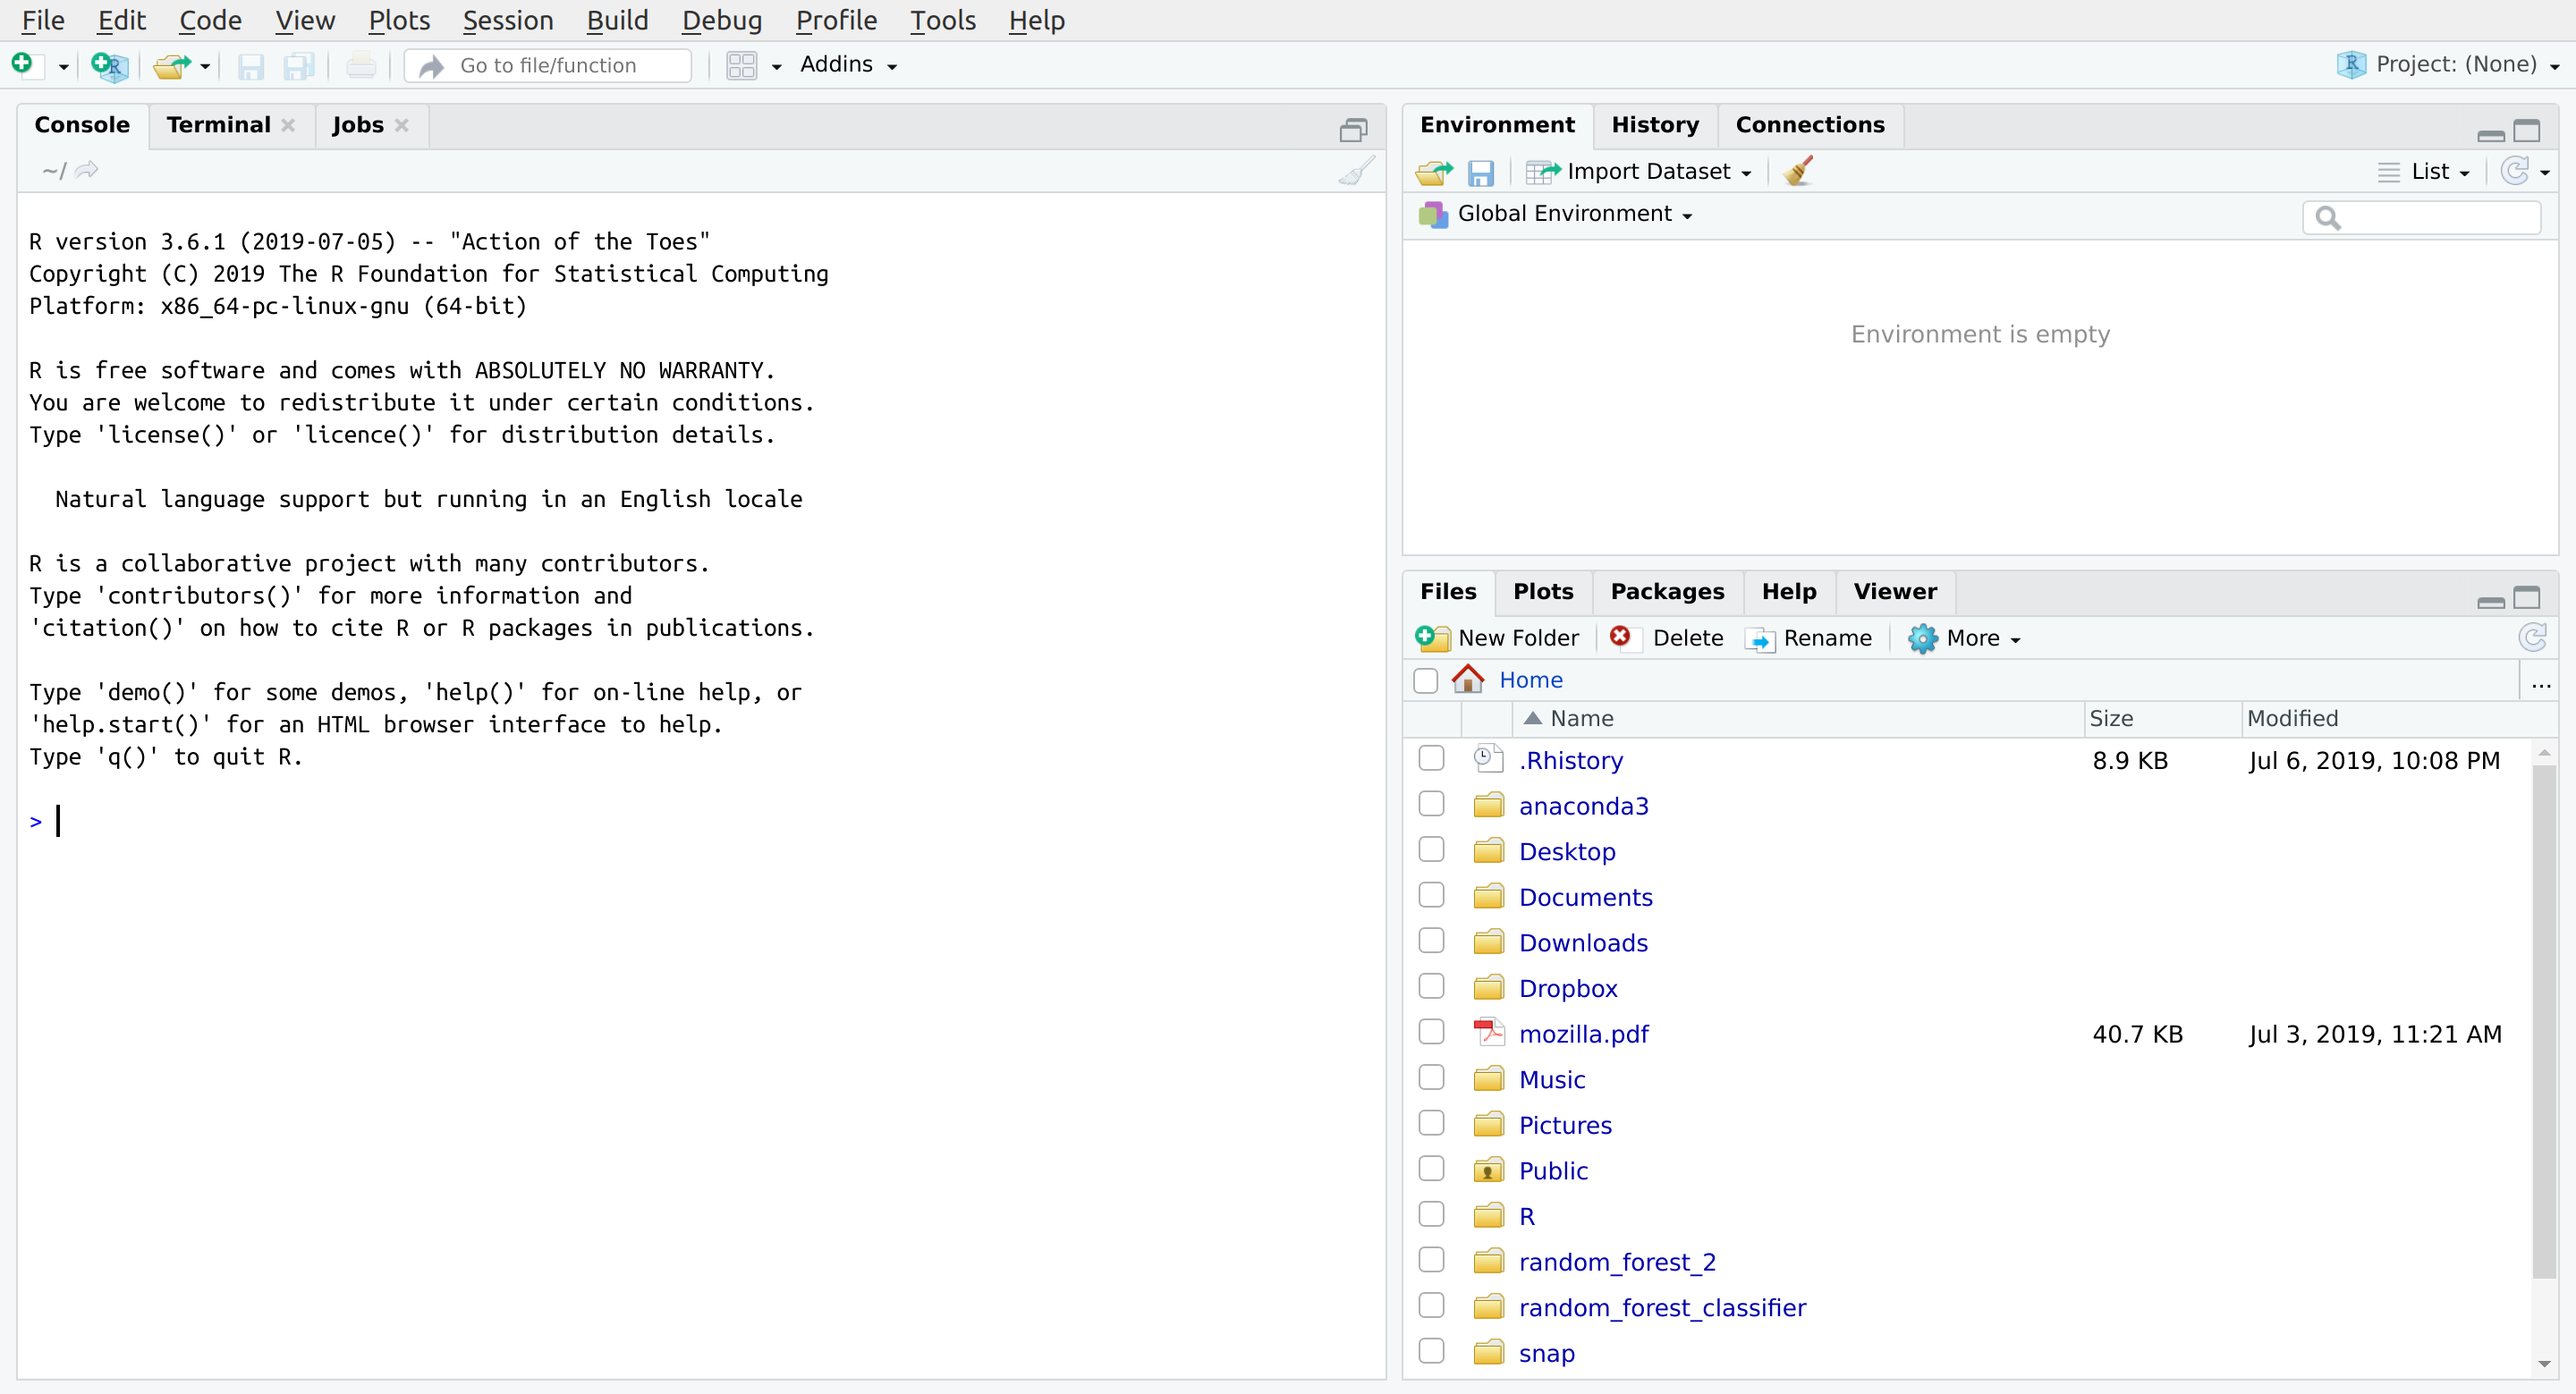
\includegraphics[width=40in]{images/RStudio1} 

}

\caption{La primera vez que abres RStudio}\label{fig:fig-main}
\end{figure}

Si tu RStudio tiene sólo 3 páneles, como en mi caso, ve a la esquina superior izquierda (signo de hoja+) y elige un nuevo \texttt{R\ Script}

\begin{figure}

{\centering 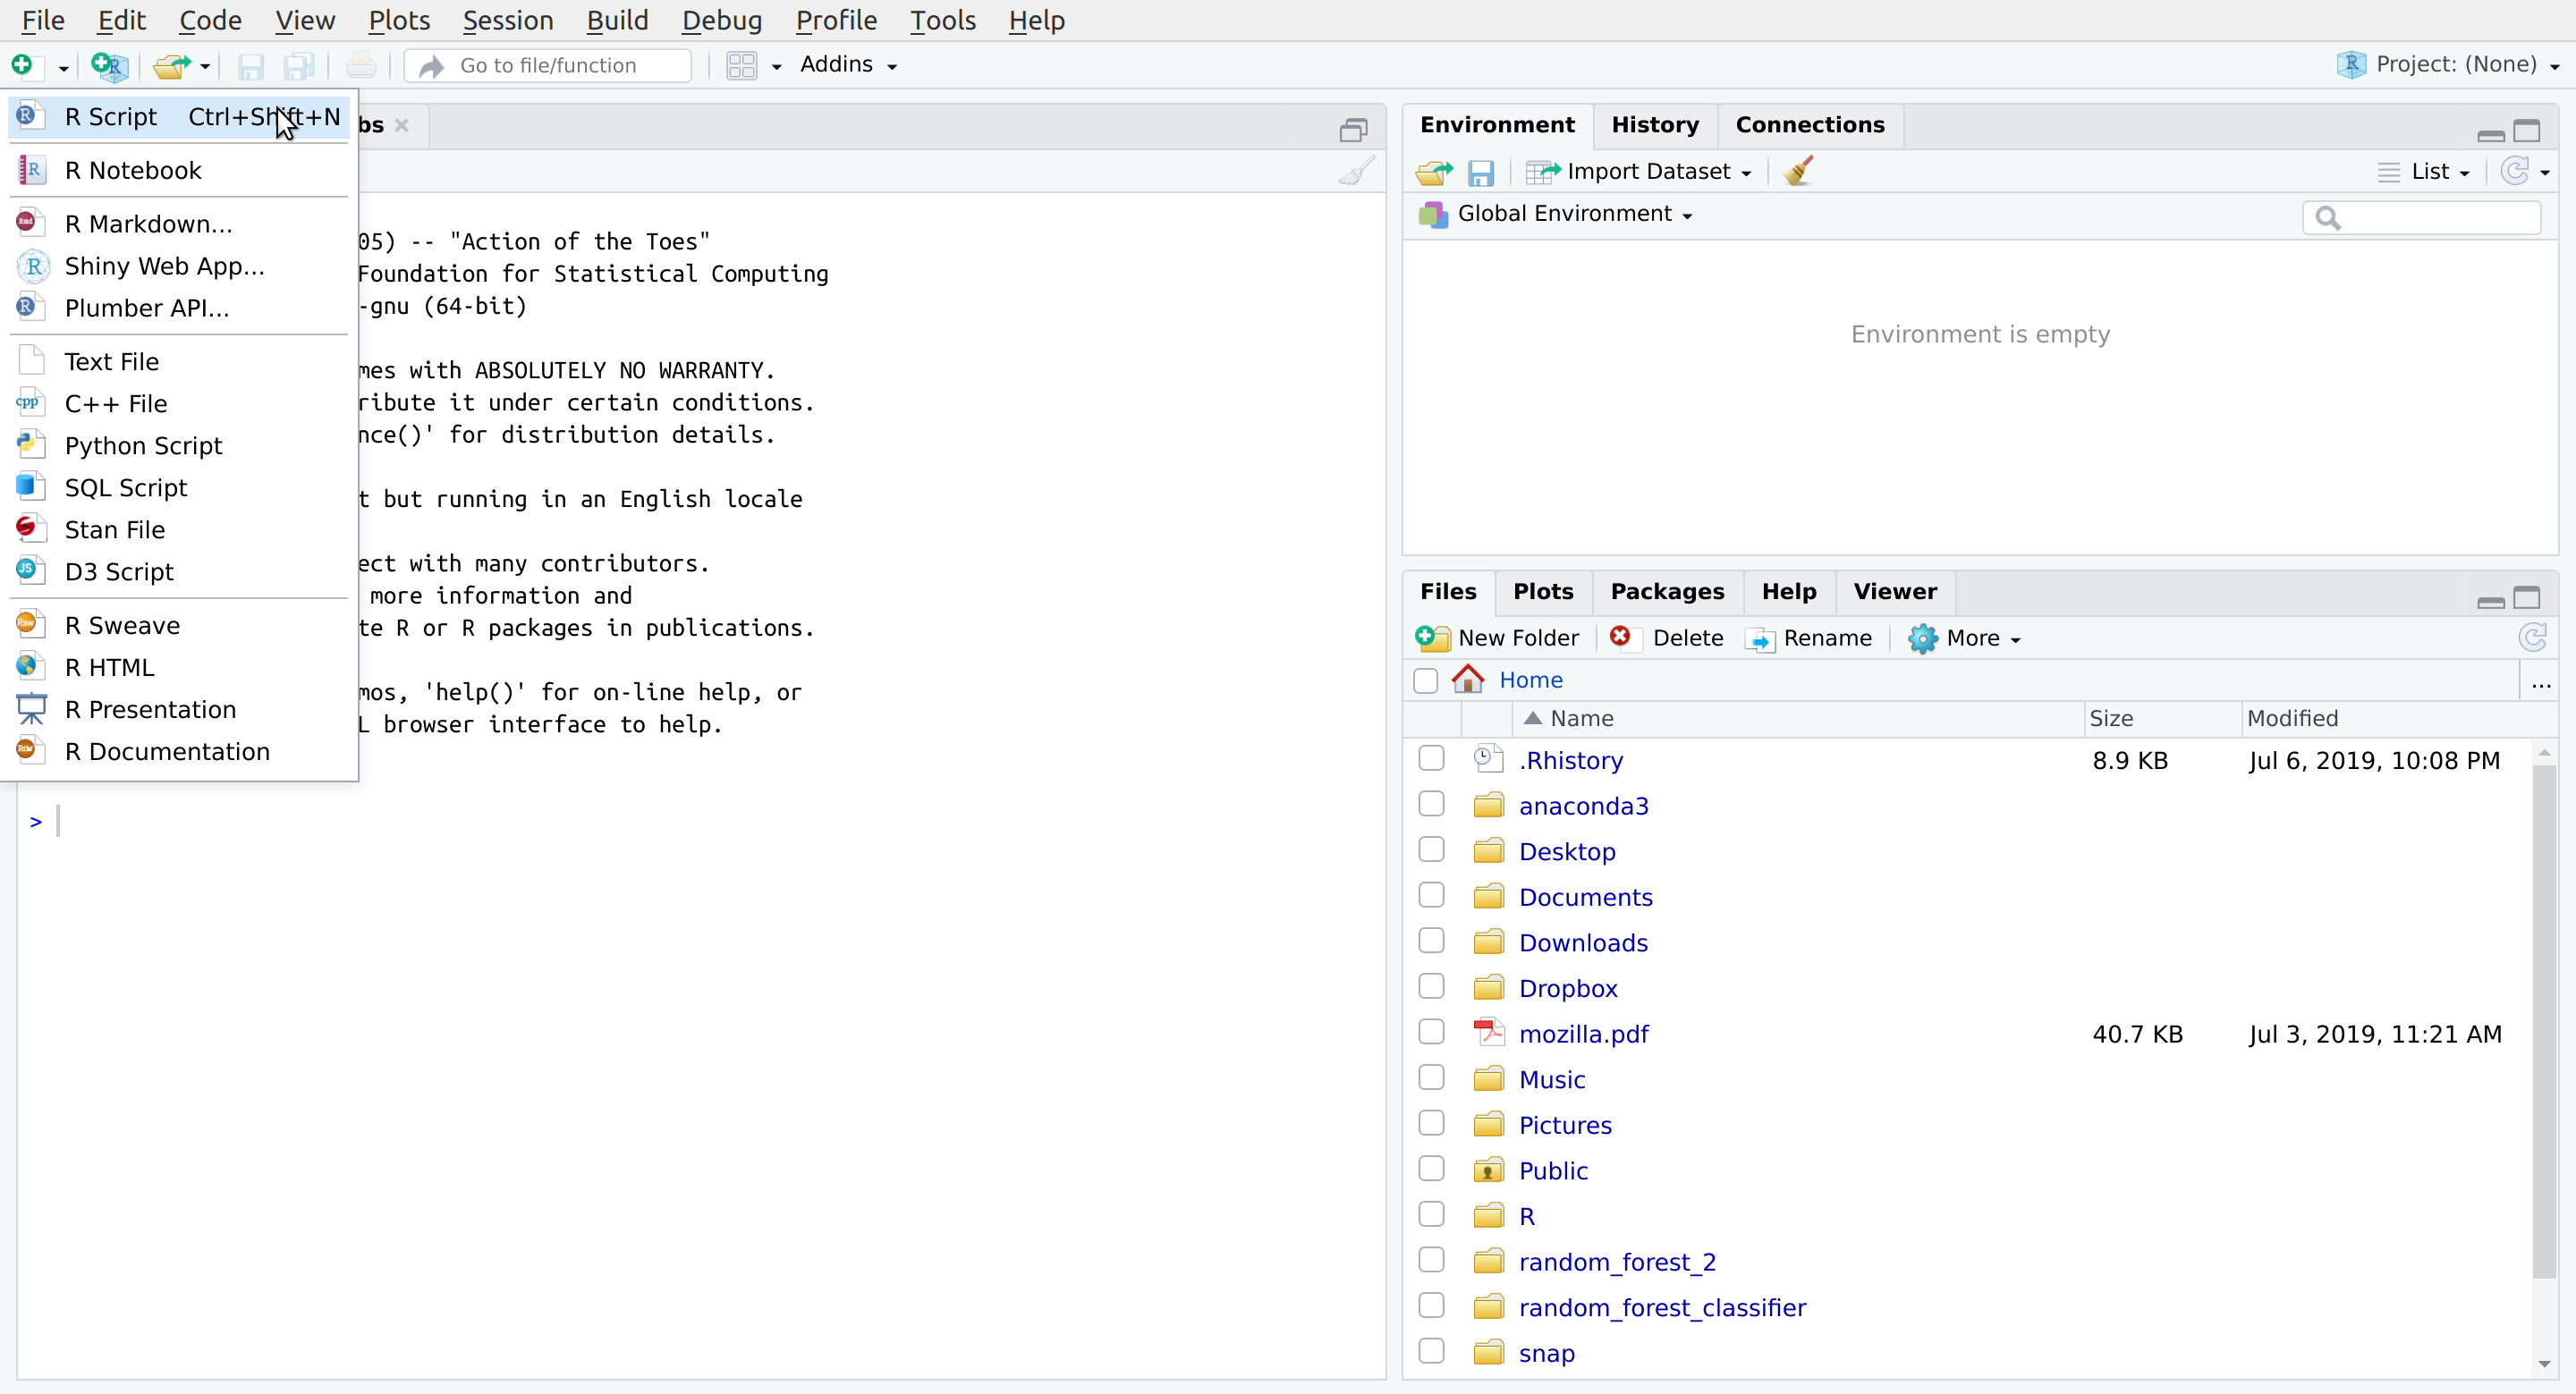
\includegraphics[width=40in]{images/RStudio2} 

}

\caption{Elige hoja+ para crear un nuevo archivo}\label{fig:unnamed-chunk-9}
\end{figure}

Tendrás, entonces, 4 páneles como se ve a continuación:

\begin{figure}

{\centering 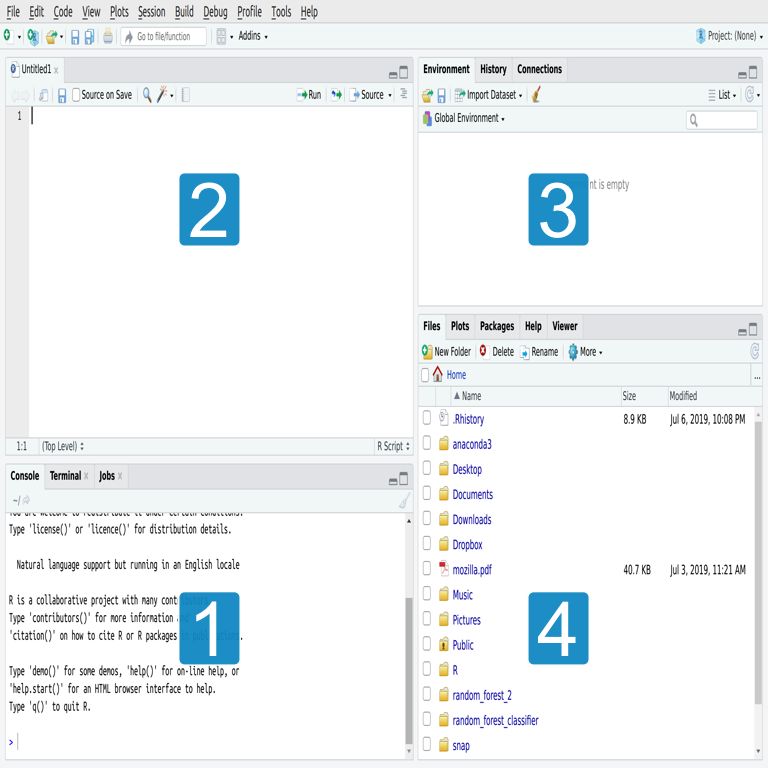
\includegraphics{Introduccion_a_Muestreo_files/figure-latex/unnamed-chunk-10-1} 

}

\caption{RStudio <3}\label{fig:unnamed-chunk-10}
\end{figure}

\begin{enumerate}
\def\labelenumi{\arabic{enumi}.}
\tightlist
\item
  El primer panel (esquina inferior izquierda) es la \texttt{Consola}. Aquí es donde se ejecutan las acciones. Prueba escribir \texttt{2\ +\ 3} en él y presiona enter. Aparece el resultado de la suma. Definitivamente, \texttt{R} es la calculadora que más trabajo cuesta instalar.
\end{enumerate}

\begin{figure}

{\centering 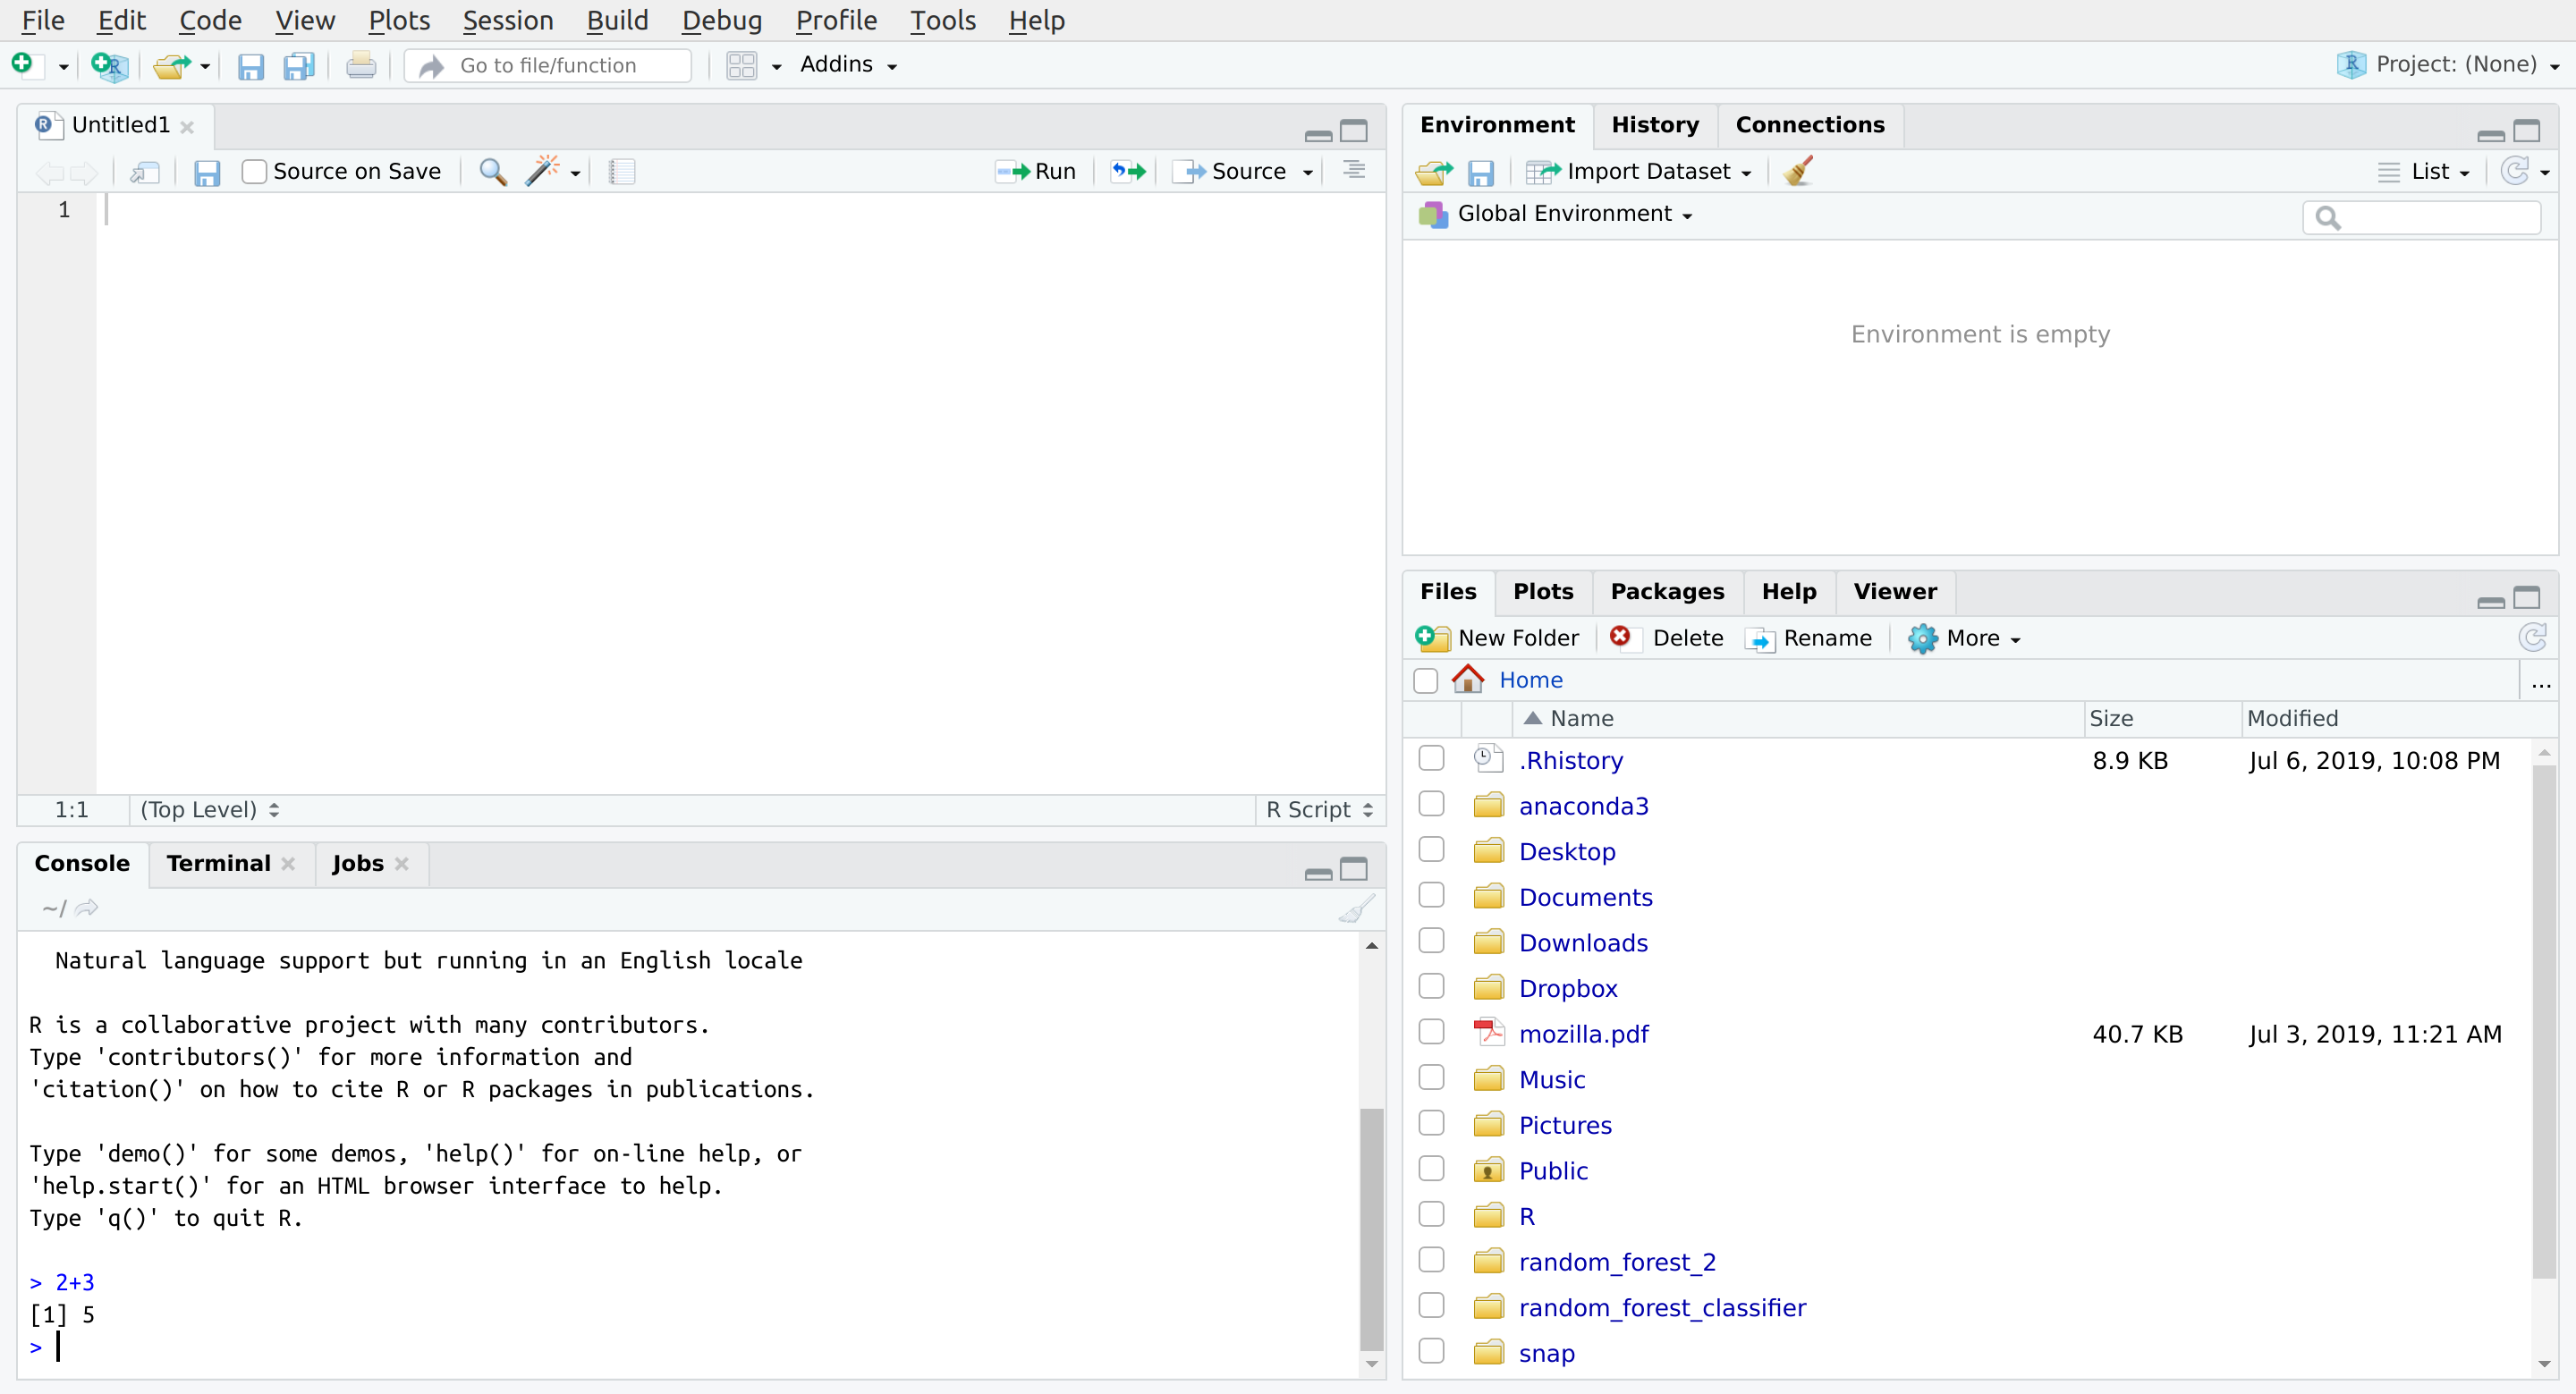
\includegraphics[width=40in]{images/RStudio4} 

}

\caption{La consola de `R` es la calculadora más difícil de instalar que existe.}\label{fig:unnamed-chunk-11}
\end{figure}

\begin{enumerate}
\def\labelenumi{\arabic{enumi}.}
\setcounter{enumi}{1}
\tightlist
\item
  El segundo panel (esquina superior izquierda) es el panel con el \texttt{Script}. Aquí se escribe el programa pero no \emph{se ejecuta}. Prueba escribir \texttt{10\ +\ 9}. ¿Ves que no pasa nada? Lo que acabas de hacer es crear un programa que, cuando se ejecute, hará la suma de \texttt{10\ +\ 9}. ¡Qué programa más aburrido! Sin embargo, no todo está perdido: presiona \texttt{CTRL+Enter} (\texttt{Cmd+Enter} en Mac) al final de la línea o bien da clic en \texttt{Run} y verás que, en la consola, aparece la instrucción y el resultado de la misma. El \texttt{Script} es una excelente fuente para tener un historial de lo que estás haciendo.
\end{enumerate}

\begin{figure}

{\centering 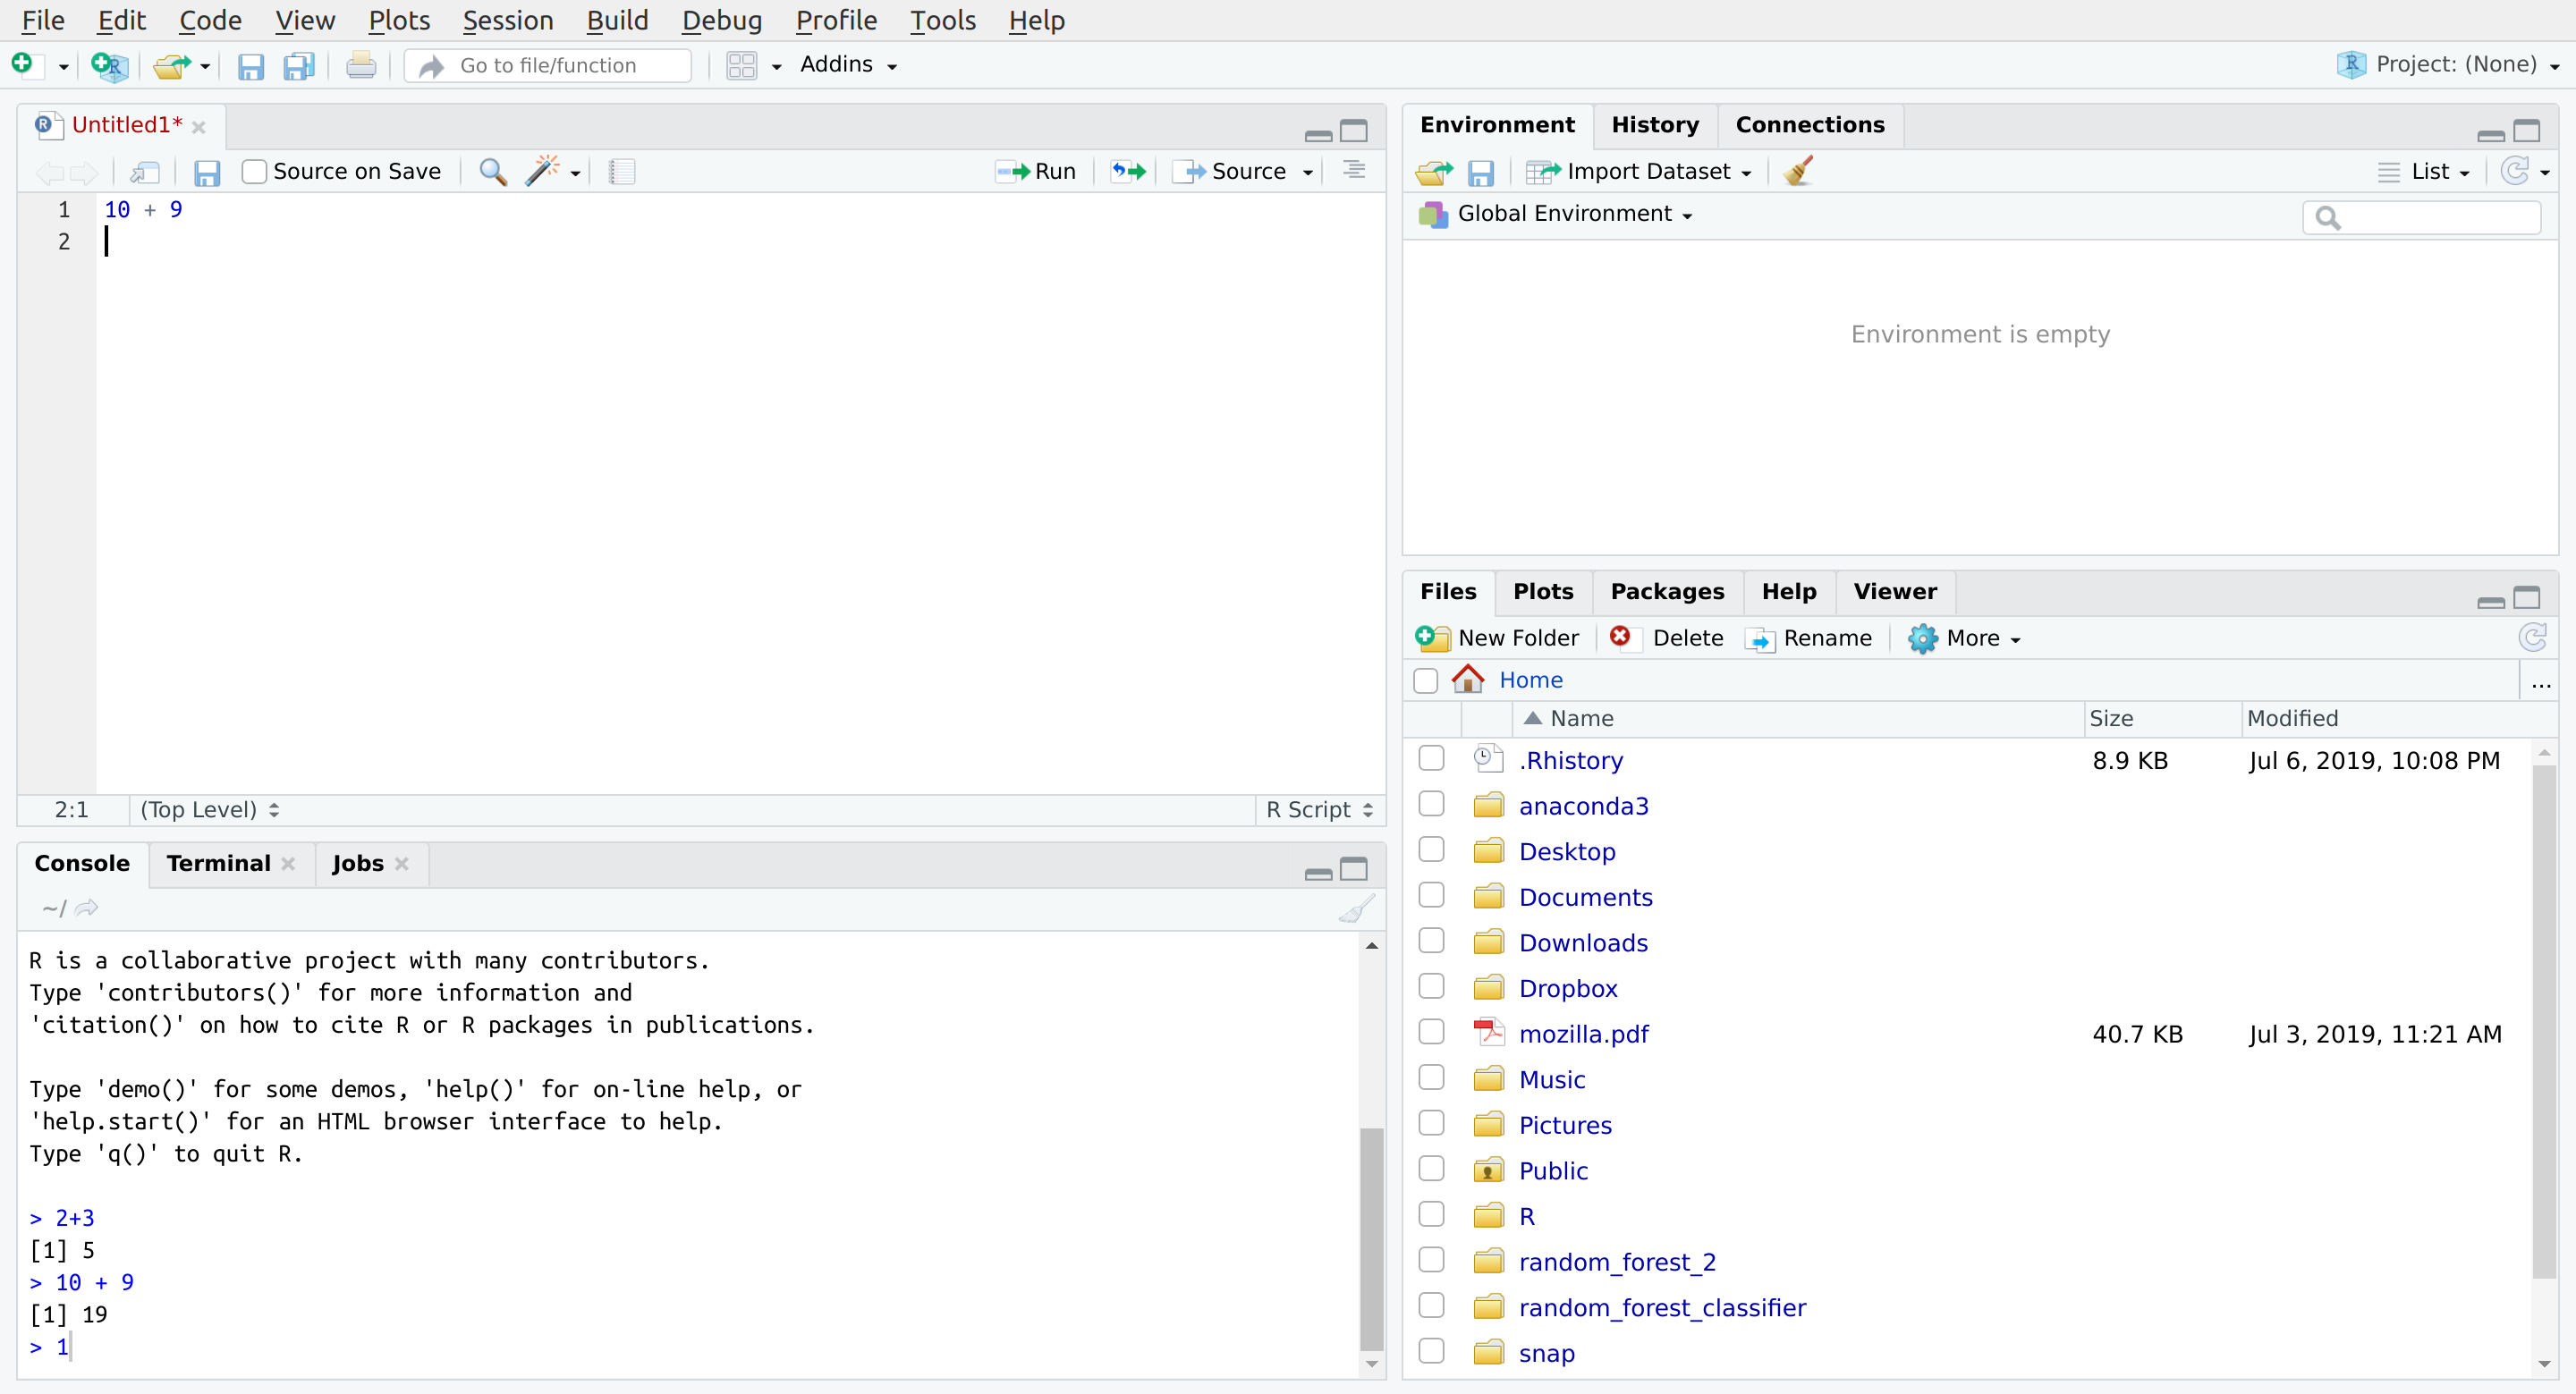
\includegraphics[width=40in]{images/RStudio5} 

}

\caption{El `Script` sirve para salvar las instrucciones en el orden en que las vas a ejecutar.}\label{fig:unnamed-chunk-12}
\end{figure}

\begin{enumerate}
\def\labelenumi{\arabic{enumi}.}
\setcounter{enumi}{2}
\tightlist
\item
  El tercer panel contiene el ambiente. Aquí aparecerán las variables que vayamos creando. Por ahora, para poner un ejemplo, importaremos el archivo \texttt{Example1.csv} (con valores simulados) dando clic en \texttt{Import\ Dataset} y \texttt{From\ Text\ (base)}. Selecciona el archivo y elige las opciones en la ventana de previsualización que hagan que se vea bien. Nota que una vez realizada la importación aparece en el panel derecho \texttt{Example1.} Al dar clic podrás ver la base de datos. Las bases de datos y variables que utilices durante tus análisis aparecerán en esa sección.
\end{enumerate}

\begin{figure}

{\centering 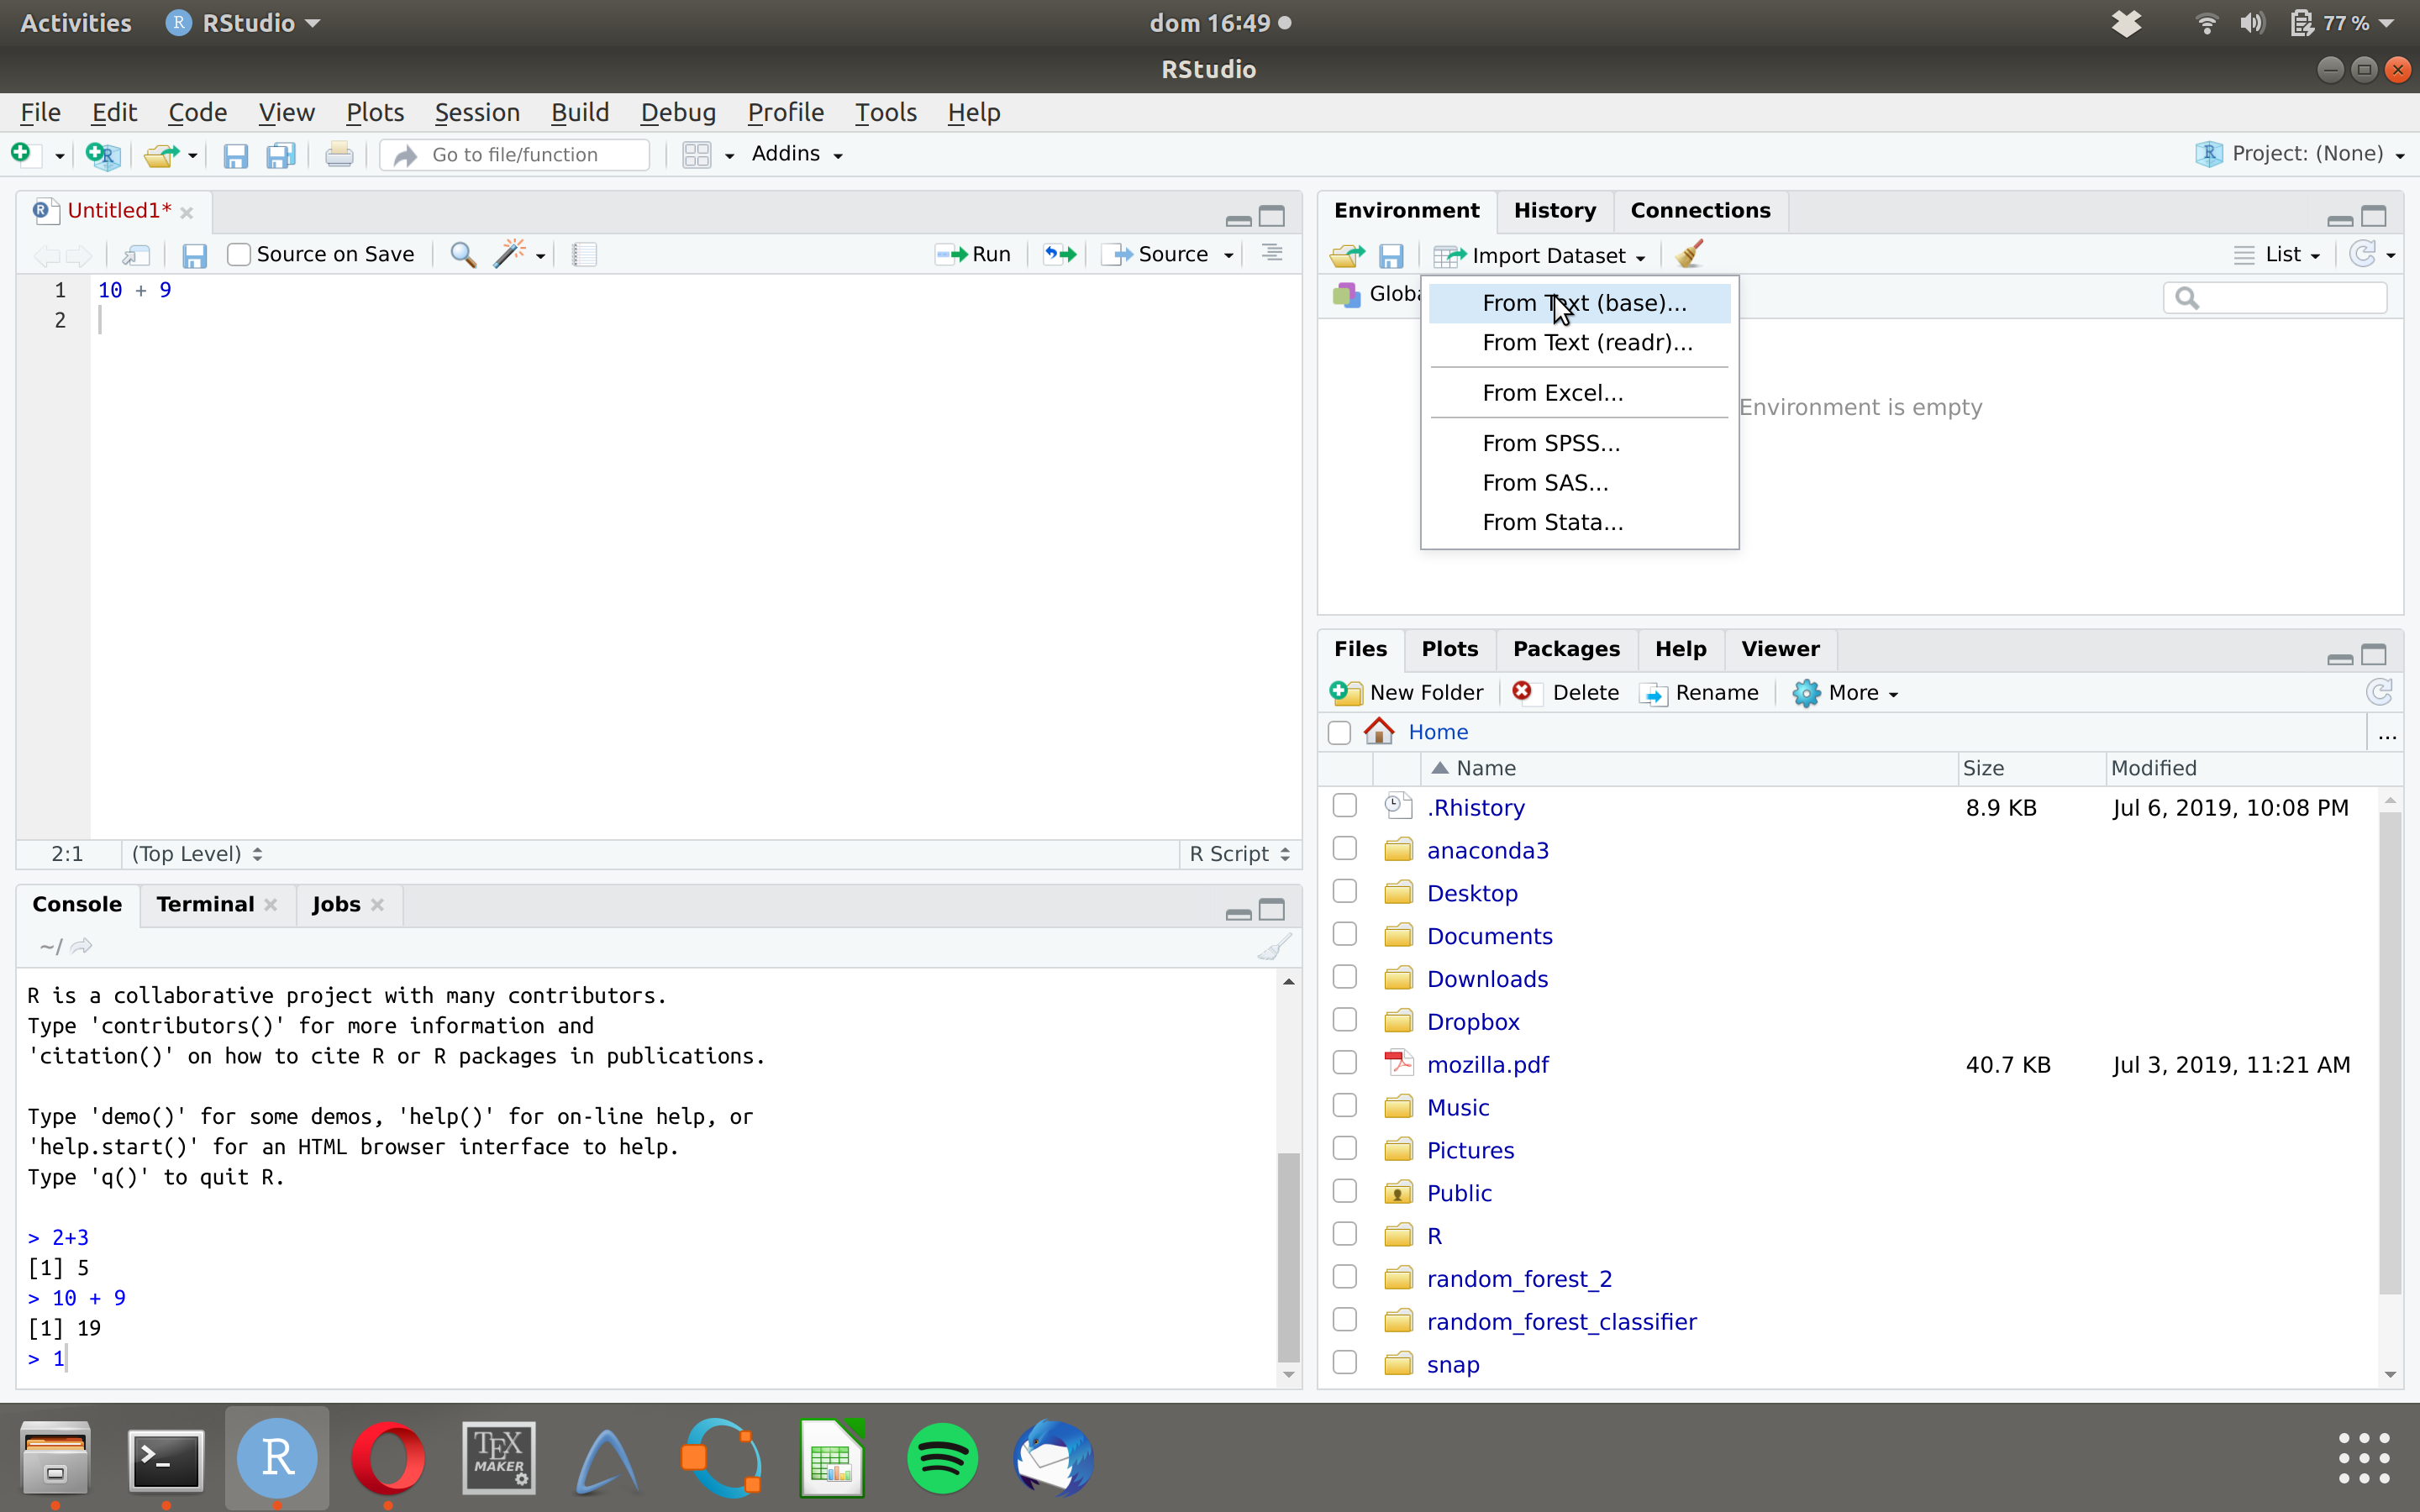
\includegraphics[width=40in]{images/RStudio6} 

}

\caption{El `Ambiente` muestra las variables (incluyendo bases de datos) que estás utilizando en este momento. A diferencia de otros programas estadísticos (o sea `Stata`) en `R` es posible tener múltiples bases de datos abiertas a la vez.}\label{fig:unnamed-chunk-14}
\end{figure}

\begin{enumerate}
\def\labelenumi{\arabic{enumi}.}
\setcounter{enumi}{3}
\tightlist
\item
  Para entender mejor lo que ocurre en el último de los páneles, lo mejor es trabajar con nuestra base. Escribe en la consola \texttt{plot(Example1)} . En el cuarto pánel aparecerá una gráfica. El cuarto de los páneles para nosotros tendrá esa utilidad: mostrará las gráficas que hagamos así como la ayuda. Para ver la ayuda para las instrucciones de \texttt{R} puedes escribir \texttt{?}. Prueba teclear \texttt{?plot} en la consola. El signo de interrogación es un \texttt{help()} que muestra las instrucciones para usar una función.
\end{enumerate}

\begin{figure}

{\centering 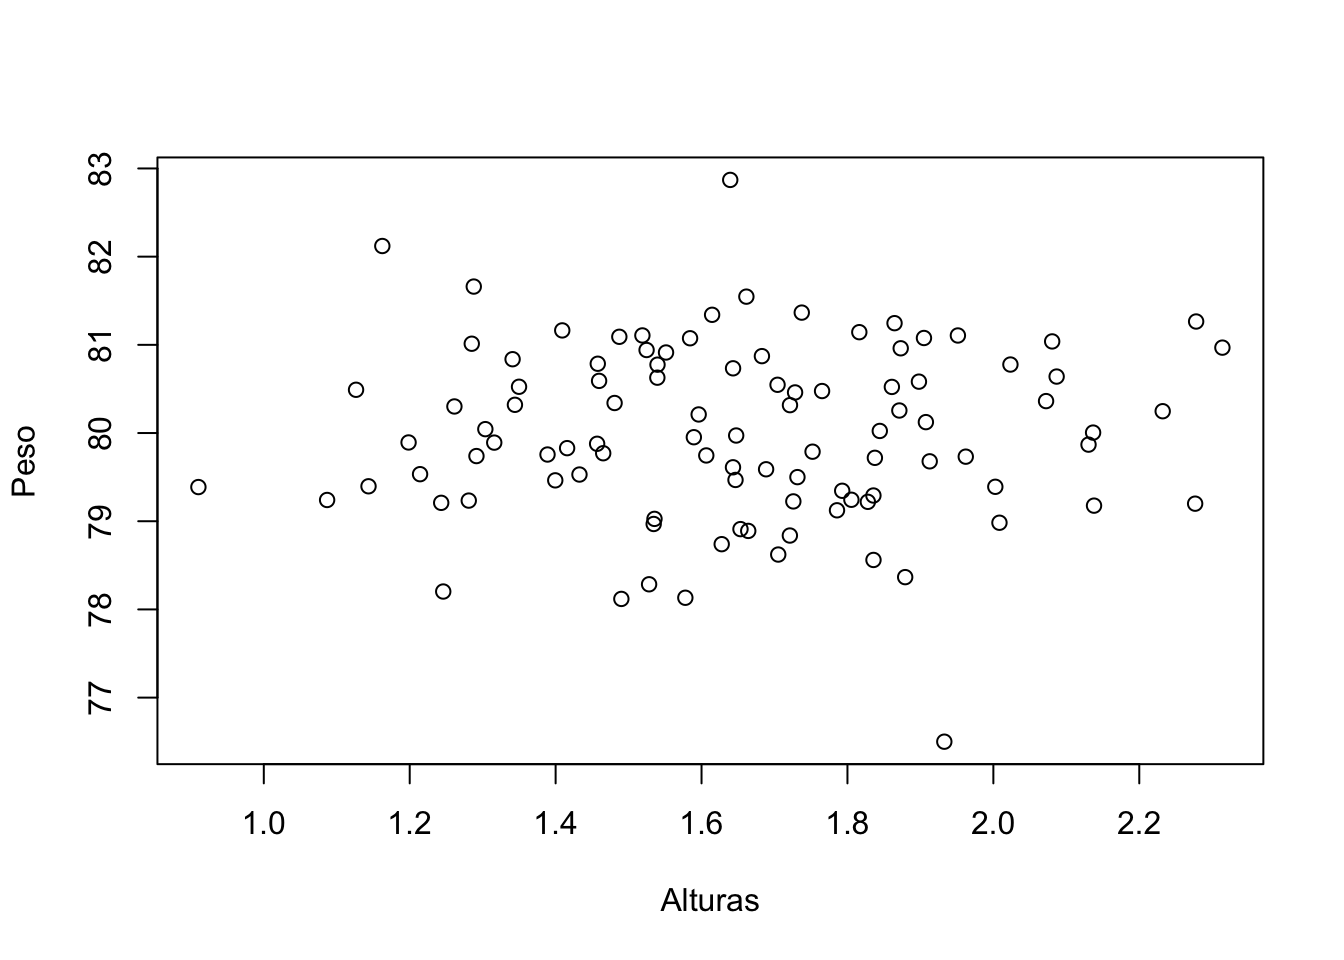
\includegraphics{Introduccion_a_Muestreo_files/figure-latex/unnamed-chunk-15-1} 

}

\caption{La gráfica que aparece de hacer un `plot` de la base de datos de ejemplo.}\label{fig:unnamed-chunk-15}
\end{figure}

\begin{figure}

{\centering 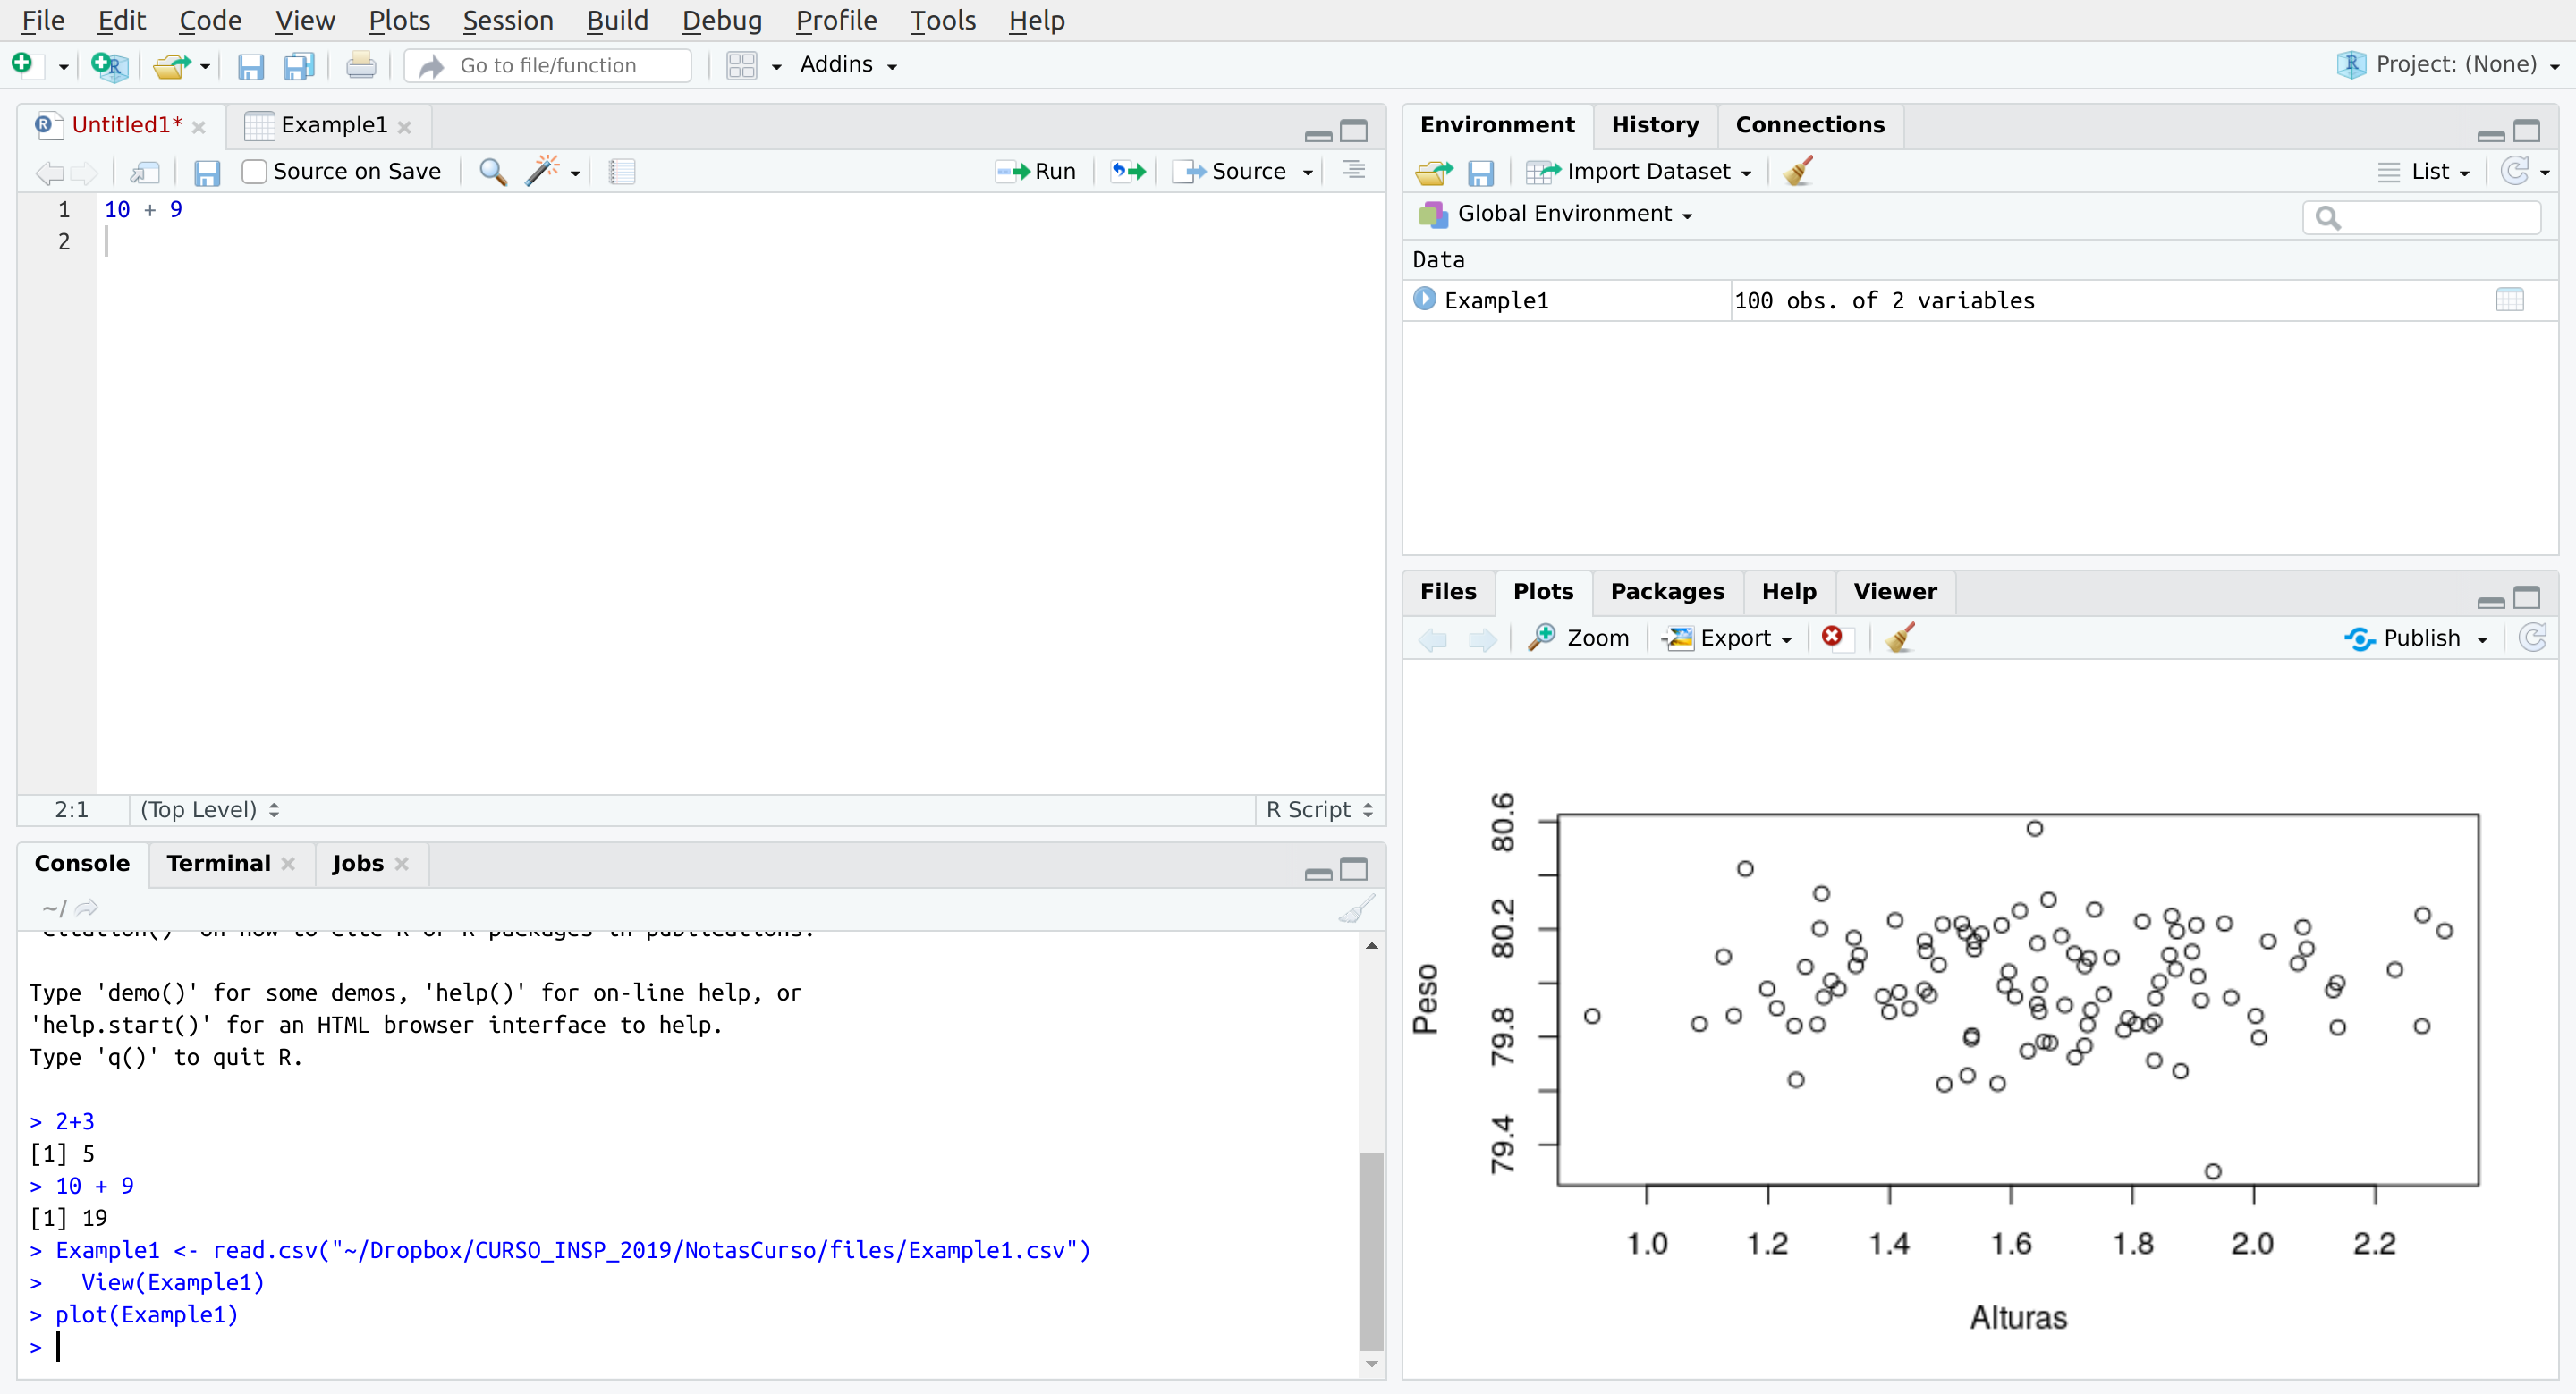
\includegraphics[width=40in]{images/RStudio7} 

}

\caption{El cuarto panel muestra respectivamente las gráficas y la ayuda.}\label{fig:unnamed-chunk-16}
\end{figure}

Mi sugerencia personal es que escribas todo lo que haces en el \texttt{Script} y que sólo utilices la consola para verificar valores. De esta manera podrás almacenar todas las instrucciones ejecutadas y volver a ellas cuando se requieran. Por último te sugiero utilizar \texttt{\#} gatos para comentar tu código. Así, el código anterior lo podrías ver en la consola como:

\begin{Shaded}
\begin{Highlighting}[]
\CommentTok{#Aquí pruebo cómo R hace las sumas}
\DecValTok{10} \OperatorTok{+}\StringTok{ }\DecValTok{9}
\end{Highlighting}
\end{Shaded}

\href{https://www.freecodecamp.org/news/code-comments-the-good-the-bad-and-the-ugly-be9cc65fbf83/}{Comenta}. \href{https://www.c-sharpcorner.com/blogs/why-comments-are-important-while-writing-a-code}{Comenta}. \href{https://blog.codinghorror.com/code-tells-you-how-comments-tell-you-why/}{Comenta, por favor}. Tu ser del futuro que regrese a sus archivos de \texttt{R} un mes después de haberlos hecho te lo agradecerá (y tu profe también).

Finalmente y como aclaración para estas notas, el código de \texttt{R} aparece como:

\begin{Shaded}
\begin{Highlighting}[]
\CommentTok{#Esto es código de R}
\DecValTok{7} \OperatorTok{-}\StringTok{ }\DecValTok{2}
\end{Highlighting}
\end{Shaded}

Mientras que los resultados de evaluar en \texttt{R} se ven con \texttt{\#}:

\begin{verbatim}
## [1] 5
\end{verbatim}

Así, la evaluación con su resultado se ve de la siguiente forma:

\begin{Shaded}
\begin{Highlighting}[]
\CommentTok{#Esto es código de R}
\DecValTok{7} \OperatorTok{-}\StringTok{ }\DecValTok{2}
\end{Highlighting}
\end{Shaded}

\begin{verbatim}
## [1] 5
\end{verbatim}

\hypertarget{cuxe1lculos-numuxe9ricos}{%
\section{Cálculos numéricos}\label{cuxe1lculos-numuxe9ricos}}

\texttt{R} sirve como calculadora para las operaciones usuales. En él puedes hacer sumas,

\begin{Shaded}
\begin{Highlighting}[]
\CommentTok{#Esto es una suma en R}
\DecValTok{12} \OperatorTok{+}\StringTok{ }\DecValTok{31}
\end{Highlighting}
\end{Shaded}

\begin{verbatim}
## [1] 43
\end{verbatim}

\begin{figure}

{\centering 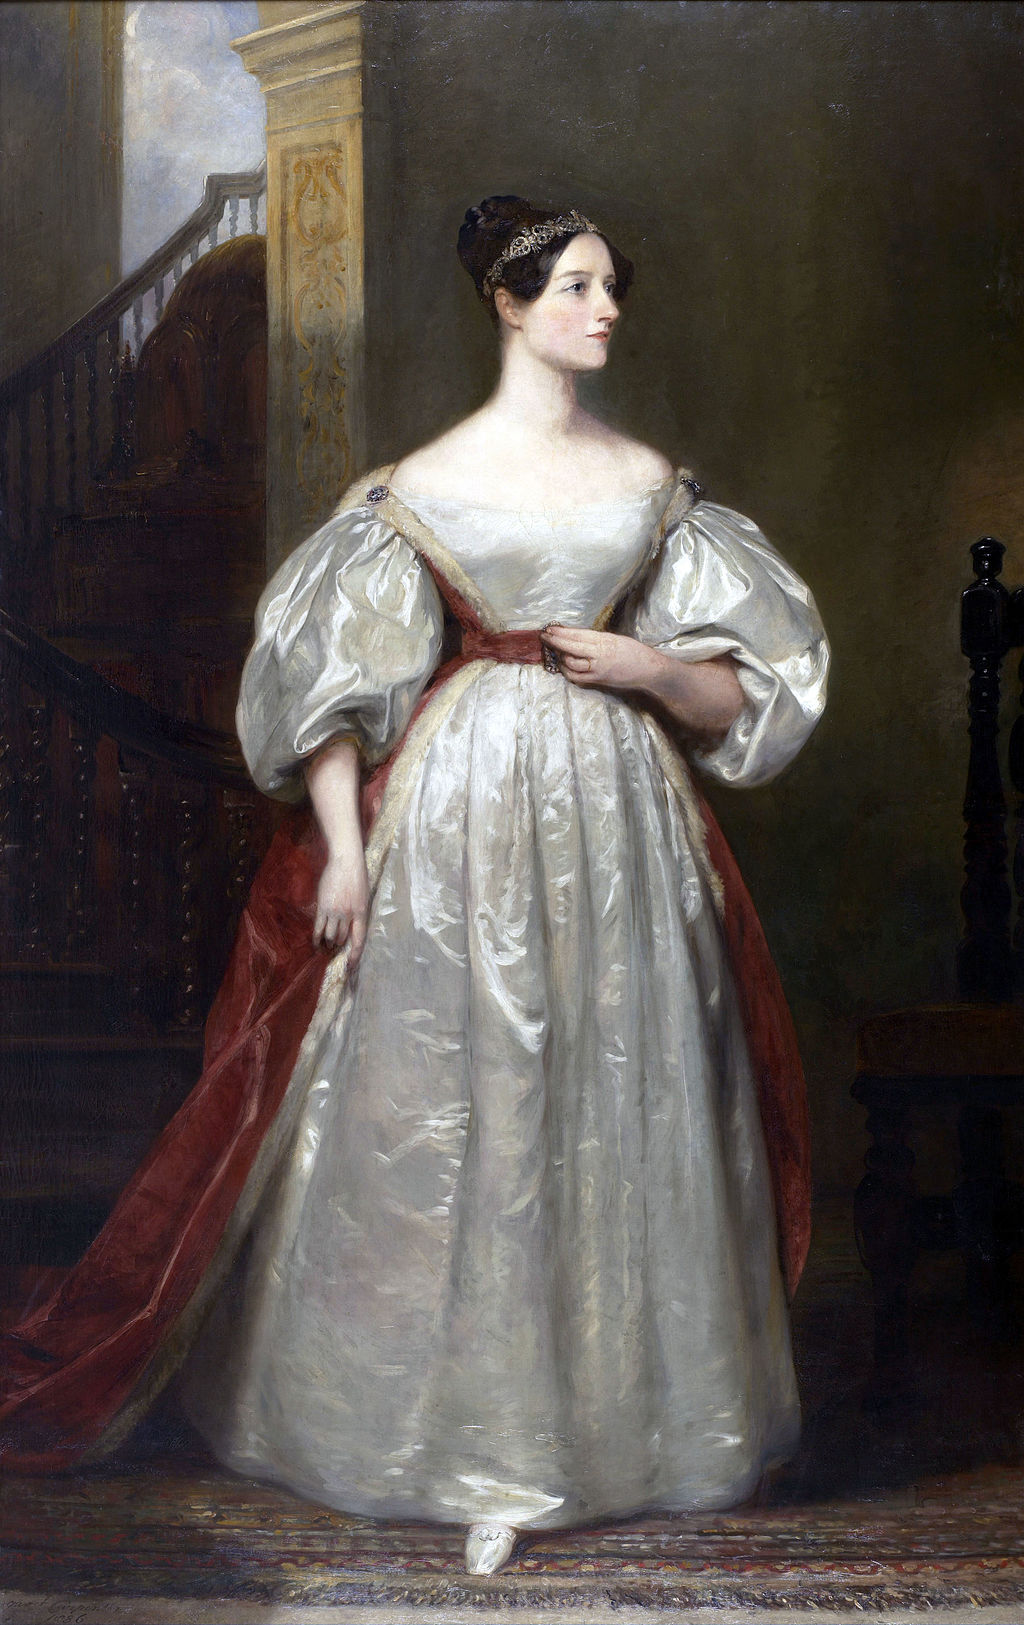
\includegraphics[width=14.22in]{images/ada_lovelace} 

}

\caption{Ada Lovelace (1815-1852), la primera en diseñar un algoritmo computacional ¡y sin tener computadoras!}\label{fig:unnamed-chunk-22}
\end{figure}

restas,

\begin{Shaded}
\begin{Highlighting}[]
\CommentTok{#Esto es una resta en R}
\DecValTok{3} \OperatorTok{-}\StringTok{ }\DecValTok{4}
\end{Highlighting}
\end{Shaded}

\begin{verbatim}
## [1] -1
\end{verbatim}

multiplicaciones,

\begin{Shaded}
\begin{Highlighting}[]
\CommentTok{#Esto es una multiplicación en R}
\DecValTok{7}\OperatorTok{*}\DecValTok{8}
\end{Highlighting}
\end{Shaded}

\begin{verbatim}
## [1] 56
\end{verbatim}

divisiones,

\begin{Shaded}
\begin{Highlighting}[]
\CommentTok{#Esto es una división en R}
\DecValTok{4}\OperatorTok{/}\DecValTok{2}
\end{Highlighting}
\end{Shaded}

\begin{verbatim}
## [1] 2
\end{verbatim}

sacar logaritmos naturales \(\ln\),

\begin{Shaded}
\begin{Highlighting}[]
\CommentTok{#Para sacar logaritmo usas el comando log}
\KeywordTok{log}\NormalTok{(}\DecValTok{100}\NormalTok{)}
\end{Highlighting}
\end{Shaded}

\begin{verbatim}
## [1] 4.60517
\end{verbatim}

o bien logaritmos en cualquier base,\footnote{Recuerda que un logaritmo base \(a\) te dice a qué potencia \(b\) tuve que elevar \(a\) para llegar a \(b\). Por ejemplo \(\log_{10}(100) = 2\) te dice que para llegar al \(100\) tuviste que hacer \(10^2\).}

\begin{Shaded}
\begin{Highlighting}[]
\CommentTok{#Puedes especificar la base del logaritmo con base }
\KeywordTok{log}\NormalTok{(}\DecValTok{100}\NormalTok{, }\DataTypeTok{base =} \DecValTok{10}\NormalTok{)}
\end{Highlighting}
\end{Shaded}

\begin{verbatim}
## [1] 2
\end{verbatim}

también puedes elevar a una potencia (por ejemplo hacer \(6^3\)),

\begin{Shaded}
\begin{Highlighting}[]
\CommentTok{#Así se calculan potencias}
\DecValTok{6}\OperatorTok{^}\DecValTok{3}
\end{Highlighting}
\end{Shaded}

\begin{verbatim}
## [1] 216
\end{verbatim}

calcular la exponencial \(e\),

\begin{Shaded}
\begin{Highlighting}[]
\CommentTok{#Para exponenciales puedes usar exp}
\KeywordTok{exp}\NormalTok{(}\DecValTok{1}\NormalTok{)}
\end{Highlighting}
\end{Shaded}

\begin{verbatim}
## [1] 2.71828
\end{verbatim}

o bien exponenciar cualquier variable \(e^{-3}\),

\begin{Shaded}
\begin{Highlighting}[]
\CommentTok{#O bien exponenciales específicas, e^-3}
\KeywordTok{exp}\NormalTok{(}\OperatorTok{-}\DecValTok{3}\NormalTok{)}
\end{Highlighting}
\end{Shaded}

\begin{verbatim}
## [1] 0.0497871
\end{verbatim}

también puedes usar el número \(\pi\).

\begin{Shaded}
\begin{Highlighting}[]
\CommentTok{#Cálculo de pi}
\NormalTok{pi}
\end{Highlighting}
\end{Shaded}

\begin{verbatim}
## [1] 3.14159
\end{verbatim}

No olvides que \texttt{R} usa el orden de las operaciones de matemáticas. Siempre es de izquierda a derecha con las siguientes excepciones:

\begin{enumerate}
\def\labelenumi{\arabic{enumi}.}
\item
  Primero se evalúa lo que está entre paréntesis.
\item
  En segundo lugar se calculan potencias.
\item
  Lo tercero en evaluarse son multiplicaciones y divisiones.
\item
  Finalmente, se realizan sumas y restas.
\end{enumerate}

Por ejemplo, en la siguiente ecuación
\[
2 - 2 \cdot \frac{(3^4 - 9)}{(5 + 4)}
\]
se resuelven primero los paréntesis \((3^4 - 9) = 81 - 9 = 72\) y \((5 + 4) = 9\); luego se resuelve la división: \(\frac{72}{9}=8\), se multiplica por el \(2\): \(2 \cdot 8\) y finalmente se hace la resta: \(2-8 = -6\).

\hypertarget{ejercicio}{%
\subsection{Ejercicio}\label{ejercicio}}

Determina, sin evaluar, los resultados de los siguientes segmentos de código:

\begin{Shaded}
\begin{Highlighting}[]
\CommentTok{#Primer ejercicio }
\NormalTok{(}\DecValTok{9} \OperatorTok{-}\StringTok{ }\DecValTok{3}\NormalTok{)}\OperatorTok{^}\DecValTok{2} \OperatorTok{*}\StringTok{ }\NormalTok{(}\DecValTok{2} \OperatorTok{-}\StringTok{ }\DecValTok{1}\NormalTok{) }\OperatorTok{-}\StringTok{ }\DecValTok{6}
\end{Highlighting}
\end{Shaded}

\begin{Shaded}
\begin{Highlighting}[]
\CommentTok{#Segundo ejercicio }
\DecValTok{6} \OperatorTok{*}\StringTok{ }\DecValTok{2} \OperatorTok{/}\StringTok{ }\NormalTok{(}\DecValTok{7} \OperatorTok{-}\StringTok{ }\DecValTok{3}\NormalTok{) }\OperatorTok{*}\StringTok{ }\DecValTok{5}
\end{Highlighting}
\end{Shaded}

\begin{Shaded}
\begin{Highlighting}[]
\CommentTok{#Tercer ejercicio }
\DecValTok{2} \OperatorTok{*}\StringTok{ }\DecValTok{3} \OperatorTok{^}\StringTok{ }\DecValTok{2} \OperatorTok{*}\StringTok{ }\DecValTok{2} \OperatorTok{/}\StringTok{ }\NormalTok{(}\DecValTok{5} \OperatorTok{-}\StringTok{ }\DecValTok{4}\NormalTok{) }\OperatorTok{*}\StringTok{ }\DecValTok{1} \OperatorTok{/}\StringTok{ }\DecValTok{10} 
\end{Highlighting}
\end{Shaded}

Evalúa para comprobar tu respuesta.

\hypertarget{ejercicio-1}{%
\subsection{Ejercicio}\label{ejercicio-1}}

Calcula el área y el perímetro de un círculo de radio 5. Recuerda que la fórmula del área es \(\pi \cdot r^2\) donde \(r\) es el radio; mientras que la del perímetro es: \(\pi \cdot d\) donde \(d\) es el díametro (= dos veces el radio).

\hypertarget{respuestas}{%
\subsection{Respuestas}\label{respuestas}}

\begin{verbatim}
## Área = 78.5398163397448
\end{verbatim}

\begin{verbatim}
## Perímetro = 31.4159265358979
\end{verbatim}

\hypertarget{variables}{%
\section{Variables}\label{variables}}

\texttt{R} es un programa orientado a objetos; esto quiere decir que \texttt{R} almacena la información en un conjunto de variables que pueden tener diferentes \texttt{clases} y opera con ellos según su clase. Por ejemplo, un conjunto de caracteres, entre comillas, es un \texttt{Character} (\texttt{R} lo piensa como texto)

\begin{Shaded}
\begin{Highlighting}[]
\CommentTok{#Un conjunto de caracteres es un char}
\StringTok{"Hola"}
\end{Highlighting}
\end{Shaded}

\begin{verbatim}
## [1] "Hola"
\end{verbatim}

Un número (por ejemplo \texttt{2} tiene clase \texttt{numeric})\footnote{Puede ser \texttt{float}, \texttt{int}, \texttt{double} pero no nos preocuparemos por eso.}. Hay que tener mucho cuidado con combinar floats con \texttt{Strings}:

\begin{Shaded}
\begin{Highlighting}[]
\CommentTok{#Código que sí funciona porque ambos son números}
\DecValTok{2} \OperatorTok{+}\StringTok{ }\DecValTok{4} 
\end{Highlighting}
\end{Shaded}

\begin{verbatim}
## [1] 6
\end{verbatim}

\begin{figure}

{\centering 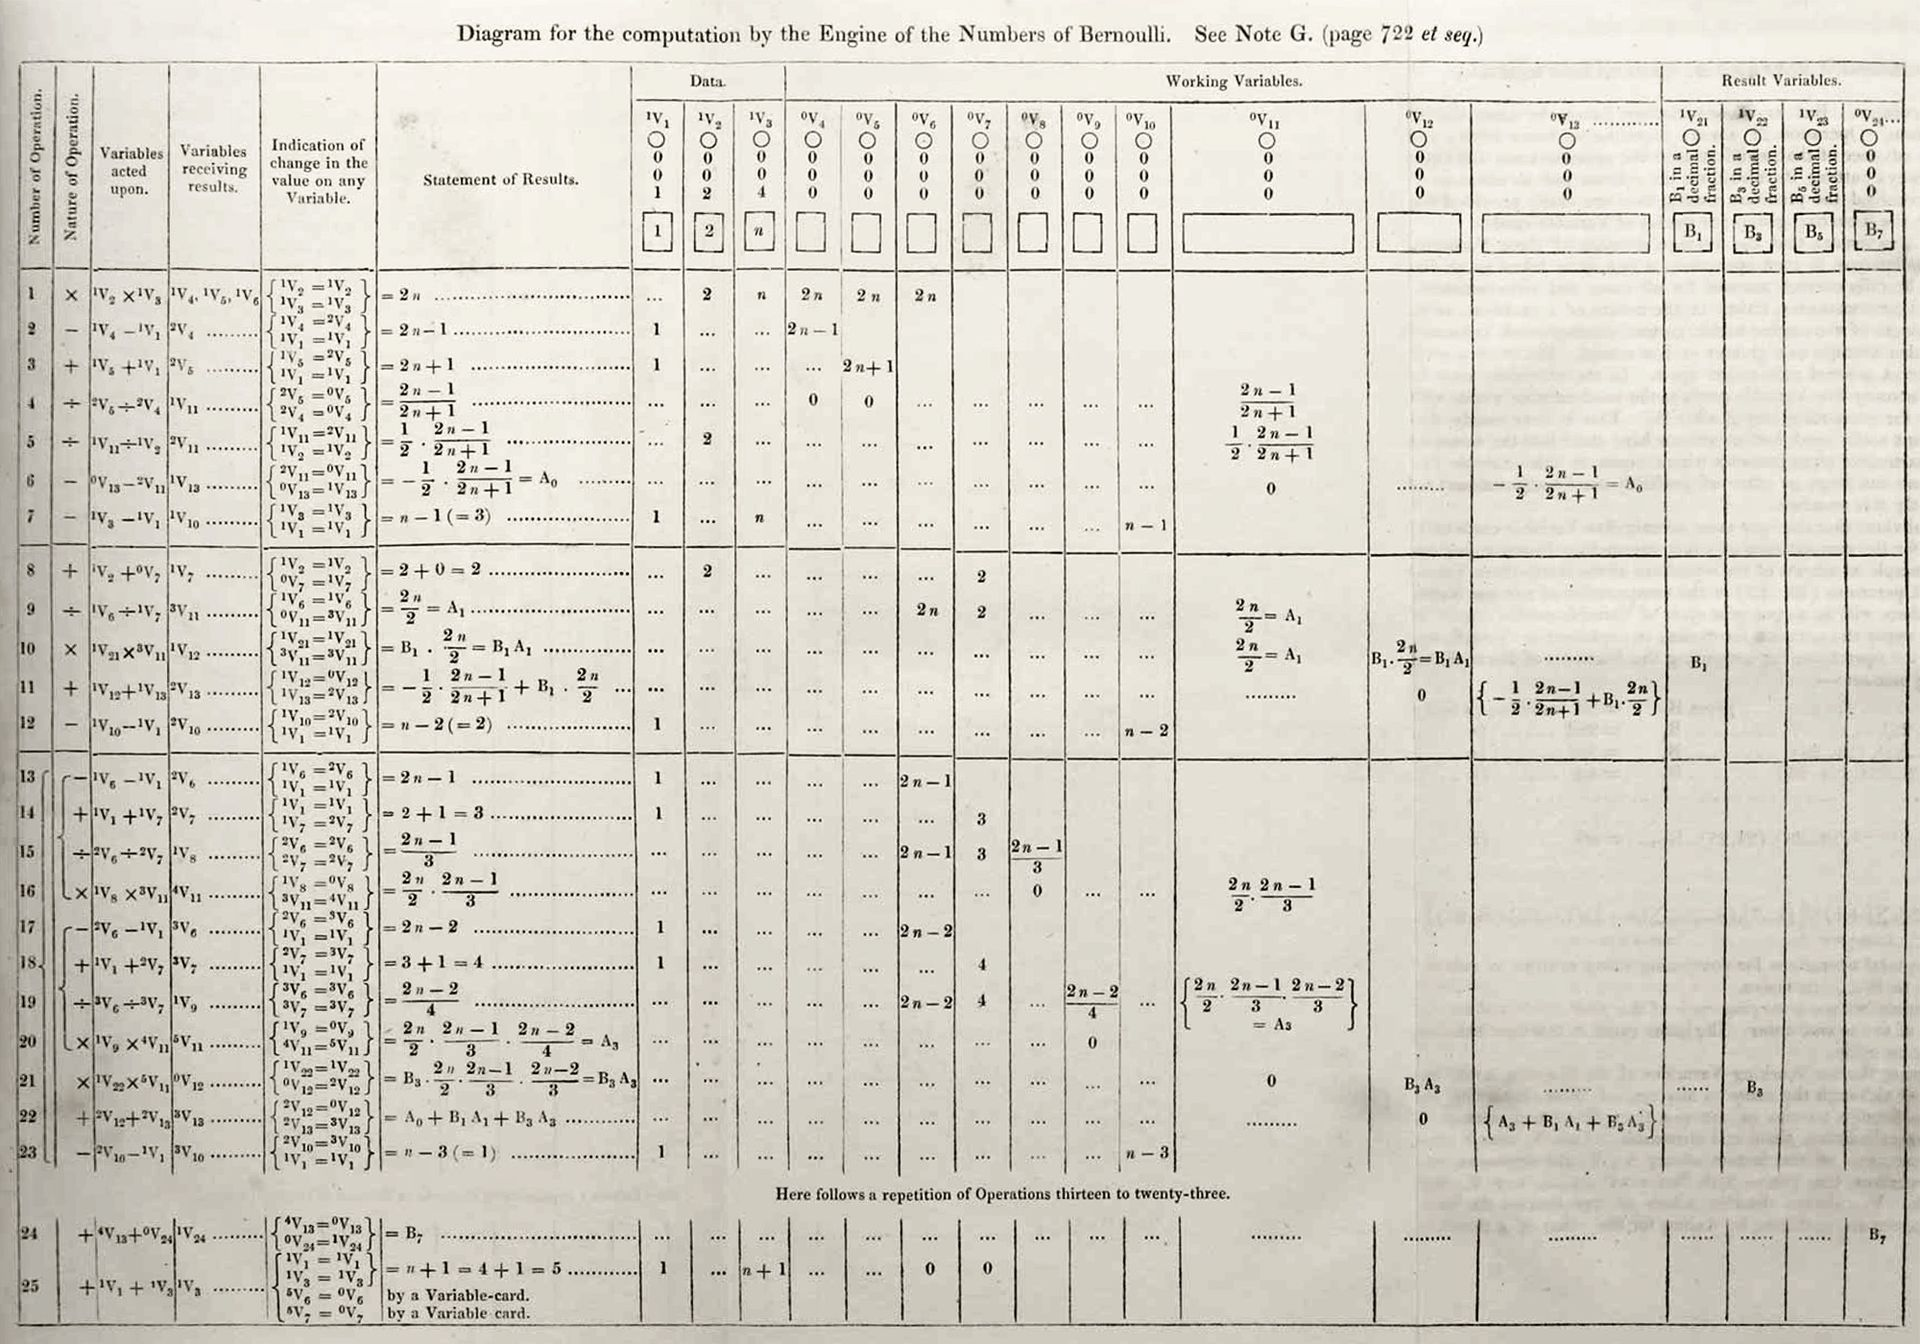
\includegraphics[width=26.67in]{images/algorithm_lovelace} 

}

\caption{El algoritmo diseñado por Ada Lovelace.}\label{fig:unnamed-chunk-38}
\end{figure}

\begin{Shaded}
\begin{Highlighting}[]
\CommentTok{#Código que no funciona porque uno es caracter}
\DecValTok{2} \OperatorTok{+}\StringTok{ "4"} 
\end{Highlighting}
\end{Shaded}

\begin{verbatim}
## Error in 2 + "4": non-numeric argument to binary operator
\end{verbatim}

Si lo piensas, este último error ¡tiene todo el sentido! no puedes sumar un número a un texto. ¿O qué significaría \texttt{\textquotesingle{}Felices\textquotesingle{}\ *\ 4} ?

La magia de \texttt{R} comienza con que puedes almacenar valores en variables. Por ejemplo, podemos asignar un valor a una variable:

\begin{Shaded}
\begin{Highlighting}[]
\CommentTok{#Asignamos x = 10}
\NormalTok{x <-}\StringTok{ }\DecValTok{10}
\end{Highlighting}
\end{Shaded}

Hay dos formas de asignar valores, una es con la flecha de asignación \(\leftarrow\) y otra con el signo de igual:

\begin{Shaded}
\begin{Highlighting}[]
\CommentTok{#Podemos asignar valores con el signo de =}
\NormalTok{y =}\StringTok{ }\DecValTok{6}
\end{Highlighting}
\end{Shaded}

Nota que, cuando realizamos operaciones, la asignación es la última que se realiza:

\begin{Shaded}
\begin{Highlighting}[]
\CommentTok{#Aquí z = 106}
\NormalTok{z <-}\StringTok{ }\NormalTok{y }\OperatorTok{+}\StringTok{ }\NormalTok{x}\OperatorTok{^}\DecValTok{2}
\end{Highlighting}
\end{Shaded}

Los valores que fueron asignados en las variables, \texttt{R} los recuerda y es posible calcular con ellos:

\begin{Shaded}
\begin{Highlighting}[]
\CommentTok{#Podemos realizar una suma}
\NormalTok{x }\OperatorTok{+}\StringTok{ }\NormalTok{y}
\end{Highlighting}
\end{Shaded}

\begin{verbatim}
## [1] 16
\end{verbatim}

\begin{Shaded}
\begin{Highlighting}[]
\CommentTok{#O bien podemos realizar una multiplicación}
\DecValTok{3}\OperatorTok{*}\NormalTok{y }\OperatorTok{-}\StringTok{ }\NormalTok{x}
\end{Highlighting}
\end{Shaded}

\begin{verbatim}
## [1] 8
\end{verbatim}

Podemos preguntarnos por el valor de las variables numéricas mediante los operadores \texttt{==} (sí, son dos iguales), \texttt{!=} (que es un \(\neq\)) \texttt{\textgreater{}}, \texttt{\textgreater{}=}, \texttt{\textless{}=} y \texttt{\textless{}}:

\begin{Shaded}
\begin{Highlighting}[]
\CommentTok{#Podemos preguntarnos si x vale 4}
\NormalTok{x }\OperatorTok{==}\StringTok{ }\DecValTok{4}
\end{Highlighting}
\end{Shaded}

\begin{verbatim}
## [1] FALSE
\end{verbatim}

\begin{quote}
El operador de asignación también se puede utilizar al revés \(2 \rightarrow x\) pero no lo hagas, por favor.
\end{quote}

Nota que no estamos asignando el valor de \texttt{x}:

\begin{Shaded}
\begin{Highlighting}[]
\NormalTok{x}
\end{Highlighting}
\end{Shaded}

\begin{verbatim}
## [1] 10
\end{verbatim}

Podemos preguntarnos por diferencia:

\begin{Shaded}
\begin{Highlighting}[]
\NormalTok{x }\OperatorTok{!=}\StringTok{ }\DecValTok{4} 
\end{Highlighting}
\end{Shaded}

\begin{verbatim}
## [1] TRUE
\end{verbatim}

Así como por mayores, menores incluyendo posibles igualdades (\emph{i.e.} los casos \(\geq\) y \(\leq\))

\begin{Shaded}
\begin{Highlighting}[]
\CommentTok{#Nos preguntamos si x > y}
\NormalTok{x }\OperatorTok{>}\StringTok{ }\NormalTok{y}
\end{Highlighting}
\end{Shaded}

\begin{verbatim}
## [1] TRUE
\end{verbatim}

\begin{Shaded}
\begin{Highlighting}[]
\CommentTok{#Nos preguntamos si x >= 10}
\NormalTok{x }\OperatorTok{>=}\StringTok{ }\DecValTok{10}
\end{Highlighting}
\end{Shaded}

\begin{verbatim}
## [1] TRUE
\end{verbatim}

\begin{Shaded}
\begin{Highlighting}[]
\CommentTok{#Nos preguntamos si y < 6}
\NormalTok{y }\OperatorTok{<}\StringTok{ }\DecValTok{6}
\end{Highlighting}
\end{Shaded}

\begin{verbatim}
## [1] FALSE
\end{verbatim}

\begin{Shaded}
\begin{Highlighting}[]
\CommentTok{#O bien si y <= 6}
\NormalTok{y }\OperatorTok{<=}\StringTok{ }\DecValTok{6}
\end{Highlighting}
\end{Shaded}

\begin{verbatim}
## [1] TRUE
\end{verbatim}

En todos los casos los resultados han sido \texttt{TRUE} ó \texttt{FALSE}. La clase de variables que toma valores \texttt{TRUE} ó \texttt{FALSE} se conoce como booleana. Hay que tener mucho cuidado con ellas porque, puedes acabar con resultados muy extraños:

\begin{Shaded}
\begin{Highlighting}[]
\CommentTok{#MALAS PRÁCTICAS, NO HAGAS ESTO}
\CommentTok{#Cuando lo usas como número TRUE vale 1}
\DecValTok{100} \OperatorTok{+}\StringTok{ }\OtherTok{TRUE}
\end{Highlighting}
\end{Shaded}

\begin{verbatim}
## [1] 101
\end{verbatim}

\begin{Shaded}
\begin{Highlighting}[]
\CommentTok{#MALAS PRÁCTICAS, NO HAGAS ESTO}
\CommentTok{#Cuando lo usas como número FALSE vale 0}
\DecValTok{6}\OperatorTok{*}\OtherTok{FALSE}
\end{Highlighting}
\end{Shaded}

\begin{verbatim}
## [1] 0
\end{verbatim}

\begin{quote}
\href{https://medium.com/mindorks/common-bad-programming-practices-7fb470ed74d2}{Aquí} puedes encontrar una lista de malas prácticas en computación a evitar.
\end{quote}

Finalmente, nota que es posible reescribir una variable y cambiar su valor:

\begin{Shaded}
\begin{Highlighting}[]
\CommentTok{#Aquí x vale 10, como antes}
\NormalTok{x}
\end{Highlighting}
\end{Shaded}

\begin{verbatim}
## [1] 10
\end{verbatim}

\begin{Shaded}
\begin{Highlighting}[]
\CommentTok{#Aquí cambianos el valor de x y valdrá 0.5}
\NormalTok{x <-}\StringTok{ }\FloatTok{0.5}
\NormalTok{x}
\end{Highlighting}
\end{Shaded}

\begin{verbatim}
## [1] 0.5
\end{verbatim}

\hypertarget{ejercicios}{%
\subsection{Ejercicios}\label{ejercicios}}

Determina el valor que imprime \texttt{R} en cada caso, sin que corras los siguientes pedazos de código. Después, verifica tu respuesta con \texttt{R}:

\begin{Shaded}
\begin{Highlighting}[]
\CommentTok{#Primer ejercicio}
\NormalTok{x <-}\StringTok{ }\DecValTok{100}
\NormalTok{y <-}\StringTok{ }\DecValTok{3}
\NormalTok{x }\OperatorTok{>}\StringTok{ }\NormalTok{y}
\end{Highlighting}
\end{Shaded}

\begin{Shaded}
\begin{Highlighting}[]
\CommentTok{#Segundo ejercicio}
\NormalTok{z <-}\StringTok{ }\NormalTok{(}\DecValTok{4} \OperatorTok{-}\StringTok{ }\DecValTok{2}\NormalTok{)}\OperatorTok{^}\DecValTok{3}
\NormalTok{z <-}\StringTok{ }\NormalTok{z }\OperatorTok{+}\StringTok{ }\NormalTok{z }\OperatorTok{+}\StringTok{ }\NormalTok{z}
\NormalTok{z}
\end{Highlighting}
\end{Shaded}

\begin{Shaded}
\begin{Highlighting}[]
\CommentTok{#Tercer ejercicio}
\NormalTok{x <-}\StringTok{ }\DecValTok{3}
\NormalTok{y <-}\StringTok{ }\DecValTok{2}
\NormalTok{z <-}\StringTok{ }\NormalTok{x }\OperatorTok{*}\StringTok{ }\NormalTok{y}
\NormalTok{x <-}\StringTok{ }\DecValTok{5}
\NormalTok{y <-}\StringTok{ }\DecValTok{10}
\NormalTok{z}
\end{Highlighting}
\end{Shaded}

\begin{Shaded}
\begin{Highlighting}[]
\CommentTok{#Cuarto ejercicio}
\NormalTok{variable1 <-}\StringTok{ }\DecValTok{1000}
\NormalTok{variable2 <-}\StringTok{ }\DecValTok{100}
\NormalTok{variable3 <-}\StringTok{ }\NormalTok{variable1}\OperatorTok{/}\NormalTok{variable2 }\OperatorTok{<=}\StringTok{ }\DecValTok{10}
\NormalTok{variable3}
\end{Highlighting}
\end{Shaded}

\begin{Shaded}
\begin{Highlighting}[]
\CommentTok{#Quinto ejercicio}
\StringTok{"2"} \OperatorTok{-}\StringTok{ }\DecValTok{2}
\end{Highlighting}
\end{Shaded}

\begin{Shaded}
\begin{Highlighting}[]
\CommentTok{#Sexto ejercicio}
\NormalTok{(}\FloatTok{0.1} \OperatorTok{+}\StringTok{ }\FloatTok{0.1} \OperatorTok{+}\StringTok{ }\FloatTok{0.1}\NormalTok{) }\OperatorTok{==}\StringTok{ }\FloatTok{0.3}
\end{Highlighting}
\end{Shaded}

\hypertarget{nivel-3}{%
\subsection{NIVEL 3}\label{nivel-3}}

Determina, sin correr el programa, qué regresa la consola en este caso

\begin{Shaded}
\begin{Highlighting}[]
\NormalTok{x <-}\StringTok{ }\DecValTok{2} 
\NormalTok{x <-}\StringTok{ }\DecValTok{5} \OperatorTok{+}\StringTok{ }\NormalTok{x ->}\StringTok{ }\NormalTok{y ->}\StringTok{ }\NormalTok{x}
\NormalTok{x <-}\StringTok{ }\NormalTok{x}\OperatorTok{^}\DecValTok{2}
\NormalTok{x}
\end{Highlighting}
\end{Shaded}

Comprueba con la consola tus resultados; puede que encuentres respuestas poco intuitivas.

\hypertarget{observaciones-sobre-la-aritmuxe9tica-de-punto-flotante}{%
\section{Observaciones sobre la aritmética de punto flotante}\label{observaciones-sobre-la-aritmuxe9tica-de-punto-flotante}}

Si hiciste el penúltimo ejercicio (el cual, obviamente hiciste y comprobaste con la consola) podrás haber notado una trampa. Analicemos qué ocurre; quizá hicimos mal la suma

\begin{Shaded}
\begin{Highlighting}[]
\CommentTok{#Veamos si este lado está mal}
\NormalTok{(}\FloatTok{0.1} \OperatorTok{+}\StringTok{ }\FloatTok{0.1} \OperatorTok{+}\StringTok{ }\FloatTok{0.1}\NormalTok{)}
\end{Highlighting}
\end{Shaded}

\begin{verbatim}
## [1] 0.3
\end{verbatim}

\begin{Shaded}
\begin{Highlighting}[]
\CommentTok{#O si éste es el que tiene la trampa}
\FloatTok{0.3}
\end{Highlighting}
\end{Shaded}

\begin{verbatim}
## [1] 0.3
\end{verbatim}

Aparentemente no hay nada malo ¿qué rayos le pasa a \texttt{R}? La respuesta está \href{https://www.youtube.com/watch?v=PZRI1IfStY0}{en la aritmética de punto flotante}. Podemos pedirle a \texttt{R} que nos muestre los primeros 100 dígitos de la suma \texttt{0.1\ +\ 0.1\ +\ 0.1}:

\begin{figure}

{\centering 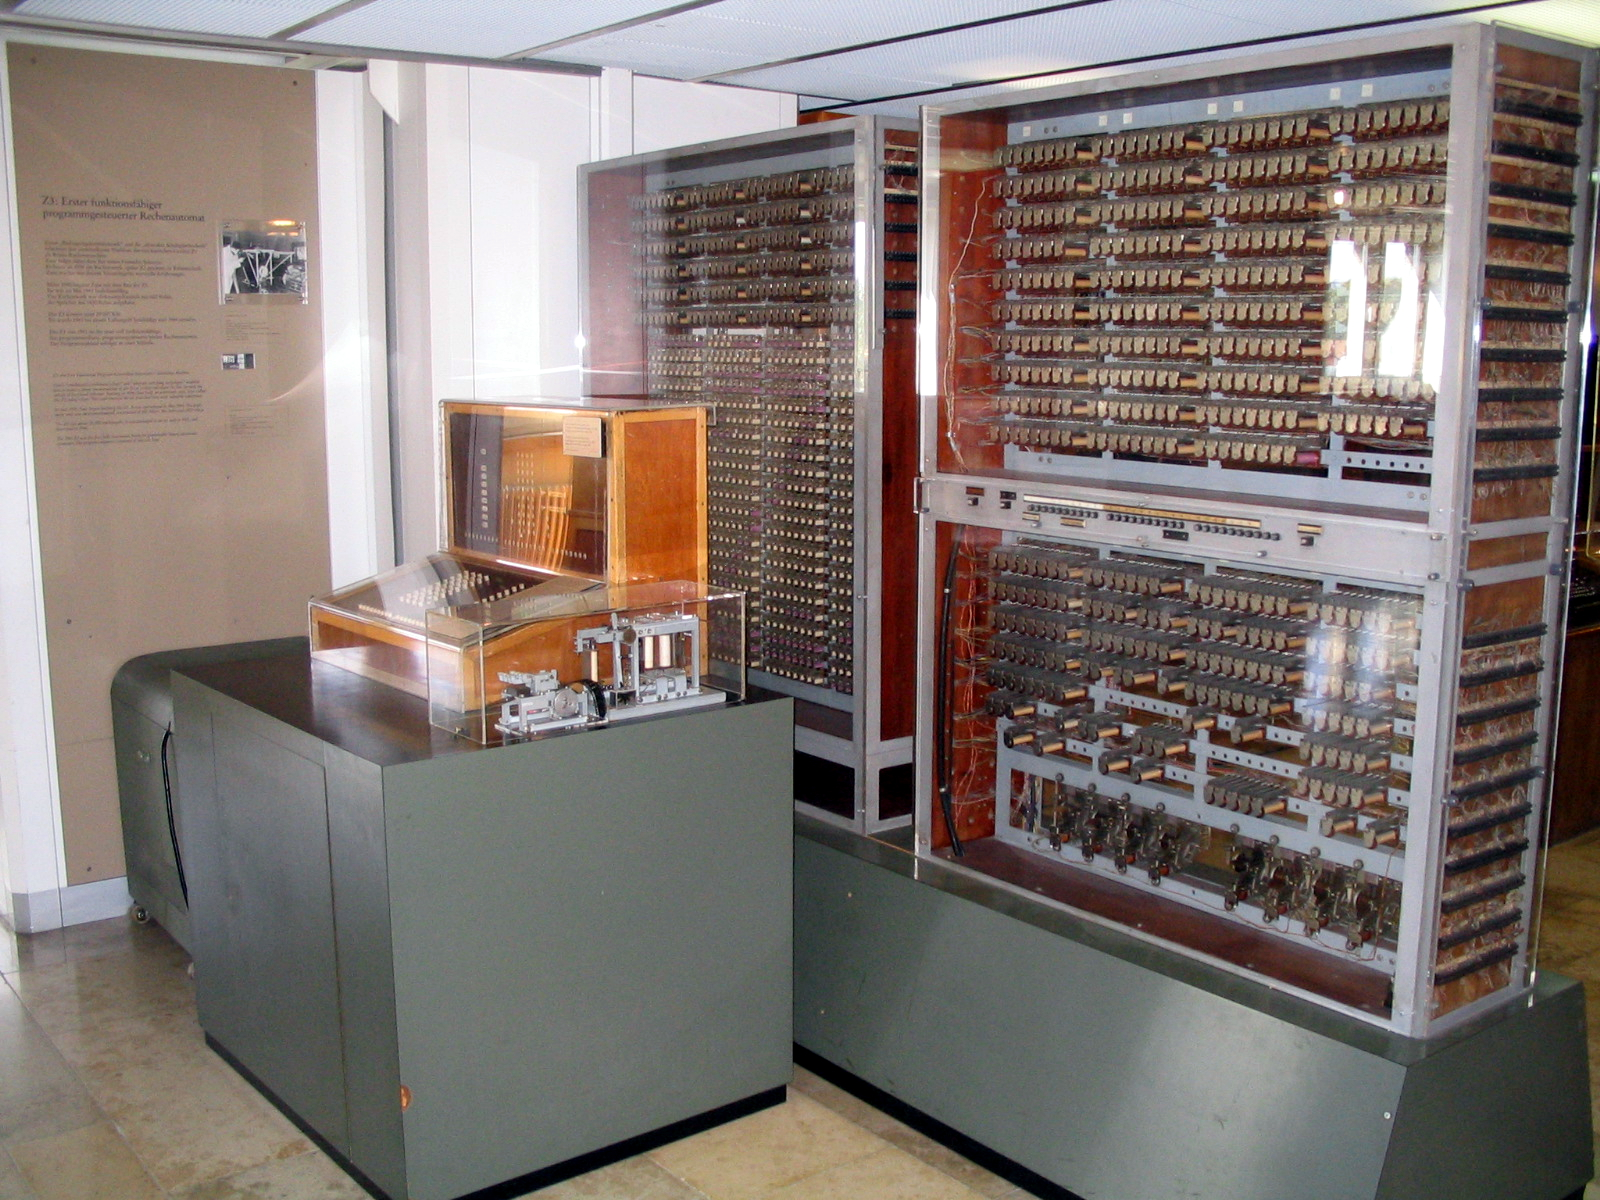
\includegraphics[width=22.22in]{images/Z3_Deutsches_Museum} 

}

\caption{Réplica de la Z3, la primer computadora con punto flotante (1941).}\label{fig:unnamed-chunk-58}
\end{figure}

\begin{Shaded}
\begin{Highlighting}[]
\CommentTok{#Veamos qué pasa con la suma}
\KeywordTok{options}\NormalTok{(}\DataTypeTok{digits =} \DecValTok{22}\NormalTok{) }\CommentTok{#Cambiamos dígitos}
\NormalTok{(}\FloatTok{0.1} \OperatorTok{+}\StringTok{ }\FloatTok{0.1} \OperatorTok{+}\StringTok{ }\FloatTok{0.1}\NormalTok{)    }\CommentTok{#Sumamos}
\end{Highlighting}
\end{Shaded}

\begin{verbatim}
## [1] 0.3000000000000000444089
\end{verbatim}

\begin{quote}
El comando \texttt{options(digits\ =\ 22)} especifica que \texttt{R} debe imprimir en la consola \texttt{22} dígitos. No más.
\end{quote}

¡\href{https://www.youtube.com/watch?v=1jaCpeXg-gg}{Ahí está el detalle}! \texttt{R} no sabe sumar. En general, ningún programa de computadora sabe hacerlo. Veamos otros ejemplos:

\begin{Shaded}
\begin{Highlighting}[]
\FloatTok{4.1} \OperatorTok{-}\StringTok{ }\FloatTok{0.1} \CommentTok{#Debería dar 4}
\end{Highlighting}
\end{Shaded}

\begin{verbatim}
## [1] 3.999999999999999555911
\end{verbatim}

\begin{Shaded}
\begin{Highlighting}[]
\DecValTok{3}\OperatorTok{/}\DecValTok{10}      \CommentTok{#Debería ser 0.3}
\end{Highlighting}
\end{Shaded}

\begin{verbatim}
## [1] 0.2999999999999999888978
\end{verbatim}

\begin{Shaded}
\begin{Highlighting}[]
\KeywordTok{log}\NormalTok{(}\DecValTok{10}\OperatorTok{^}\NormalTok{(}\DecValTok{12345}\NormalTok{), }\DataTypeTok{base =} \DecValTok{10}\NormalTok{) }\CommentTok{#Debería dar 12345}
\end{Highlighting}
\end{Shaded}

\begin{verbatim}
## [1] Inf
\end{verbatim}

El problema está en cómo las computadoras representan los números. Ellas escriben los números en binario. Por ejemplo, 230 lo representan como 11100110 mientras que el 7 es: 111. El problema de las computadoras radica en que éstas tienen una memoria finita por lo que números muy grandes como: \(124765731467098372654176\) la computadora hace lo mejor por representarlos eligiendo el más cercano:

\begin{Shaded}
\begin{Highlighting}[]
\CommentTok{#Nota la diferencia entre lo que le decimos a R}
\CommentTok{#y lo que resulta}
\NormalTok{x <-}\StringTok{ }\DecValTok{124765731467098372654176}
\NormalTok{x}
\end{Highlighting}
\end{Shaded}

\begin{verbatim}
## [1] 124765731467098377420800
\end{verbatim}

\begin{quote}
Un error de punto flotante en la vida real ocasionó en los años noventa, \href{https://www.esa.int/Newsroom/Press_Releases/Ariane_501_-_Presentation_of_Inquiry_Board_report}{la explosión del cohete \texttt{Ariane\ 5}}. Moraleja: hay que tener cuidado y respeto al punto flotante.
\end{quote}

No olvides cambiar la cantidad de dígitos que deseas que imprima \texttt{R} en su consola de vuelta:

\begin{Shaded}
\begin{Highlighting}[]
\KeywordTok{options}\NormalTok{(}\DataTypeTok{digits =} \DecValTok{6}\NormalTok{) }\CommentTok{#Cambiamos dígitos}
\end{Highlighting}
\end{Shaded}

El mismo problema ocurre con números decimales cuya representación binaria es periódica; por ejemplo el \(\frac{1}{10}\) en binario se representa como \(0.0001100110011\overline{0011}\dots\). Como es el cuento de nunca acabar con dicho número, \texttt{R} lo trunca y almacena sólo los primeros dígitos de ahí que, cada vez que escribes \texttt{0.1}, \texttt{R} en realidad almacene el 0.1000000000000000055511 que es \emph{casi lo mismo} pero no es estrictamente igual. Hay que tener mucho cuidado con esta inexactitud de las computadoras (inexactitud estudiada por la rama de \href{https://www.springer.com/gp/book/9781461484523}{Análisis Numérico}) pues puede generar varios resultados imprevistos.

\hypertarget{cuxf3mo-checar-un-if}{%
\subsection{¿Cómo checar un if?}\label{cuxf3mo-checar-un-if}}

En general lo que hacen las computadoras para comparar valores es que verifican que, en valor absoluto, el error sea pequeño. Recuerda que el valor absoluto de \(x\), \(|x|\), regresa siempre el positivo:
\[
|4| = 4 \qquad \textrm{y} \qquad |-8| = 8
\]

Para verificar que algo es más o menos \(0.3\) suele usarse el valor absoluto\footnote{En \texttt{R} el comando \texttt{abs} toma el valor absoluto.} de la siguiente manera:

\begin{Shaded}
\begin{Highlighting}[]
\KeywordTok{abs}\NormalTok{( (}\FloatTok{0.1} \OperatorTok{+}\StringTok{ }\FloatTok{0.1} \OperatorTok{+}\StringTok{ }\FloatTok{0.1}\NormalTok{) }\OperatorTok{-}\StringTok{ }\FloatTok{0.3}\NormalTok{ ) }\OperatorTok{<}\StringTok{ }\DecValTok{1}\NormalTok{.e}\DecValTok{-6}
\end{Highlighting}
\end{Shaded}

\begin{verbatim}
## [1] TRUE
\end{verbatim}

donde \texttt{1.e-6} es notación corta para 0.000001 (también escrito como \(1\times 10^{-6}\)). La pregunta que nos estamos haciendo es que si el error entre sumar \(0.1+0.1+0.1\) y \(0.3\) es muy pequeño \(< 0.000001\):
\[
| (0.1 + 0.1 + 0.1) - 0.3 | < 0.000001
\]

\hypertarget{leer-y-almacenar-variables-en-r}{%
\section{\texorpdfstring{Leer y almacenar variables en \texttt{R}}{Leer y almacenar variables en R}}\label{leer-y-almacenar-variables-en-r}}

Para terminar esta sección, aprenderemos cómo guardar variables en \texttt{R}. Para eso, el concepto de directorio es uno de los más relevantes. En general, en computación, \href{https://en.wikipedia.org/wiki/Working_directory}{el directorio} se refiere a la dirección en tu computadora donde estás trabajando. Por ejemplo, si estás en una carpeta en tu escritorio de nombre ``Ejercicios\_R'' probablemente tu directorio sea `\textasciitilde/Desktop/Ejercicios\_R/' (en Mac) o bien `\textasciitilde\textbackslash Desktop\textbackslash Ejercicios\_R\textbackslash{}' en Windows\footnote{Windows usa backslash. Y hay \href{https://www.howtogeek.com/181774/why-windows-uses-backslashes-and-everything-else-uses-forward-slashes/}{toda una historia detrás de ello}}. La forma de saber tu directorio (en general) es ir a la carpeta que te interesa y con clic derecho ver propiedades (o escribir \texttt{ls} en la terminal \texttt{Unix}).

\texttt{R} tiene un directorio \texttt{default} que quién sabe dónde está (depende de tu instalación, generalmente está donde tu \texttt{Usuario}). Usualmente lo mejor es elegir un directorio para cada uno de los proyectos que hagas. Para ello si estás en \texttt{RStudio} puedes utilizar \texttt{Shift+Ctrl+H} (\texttt{Shift+Cmd+H} en Mac) o bien ir a \texttt{Session\ \textgreater{}\ Set\ Working\ Directory\ \textgreater{}\ Choose\ Directory} y elegir el directorio donde deseas trabajar tu proyecto. Pensando que elegiste el escritorio (\texttt{Desktop} en mi computadora) notarás que en la consola aparece el comando \texttt{setwd("\textasciitilde{}/Desktop")} (o bien con `\textbackslash{}' si eres Windows). Mi sugerencia es que copies ese comando en tu \texttt{Script} para que, la próxima vez que lo corras ya tengas preestablecido el directorio.

\begin{Shaded}
\begin{Highlighting}[]
\CommentTok{#Si eres Mac/Linux}
\KeywordTok{setwd}\NormalTok{(}\StringTok{"~/Desktop"}\NormalTok{) }

\CommentTok{#Si eres Windows}
\KeywordTok{setwd}\NormalTok{(}\StringTok{"C:\textbackslash{}Users\textbackslash{}Rodrigo\textbackslash{}Desktop"}\NormalTok{) }\CommentTok{#Rodrigo = Mi usuario}
\end{Highlighting}
\end{Shaded}

Podemos verificar el directorio elegido con \texttt{getwd()}:

\begin{Shaded}
\begin{Highlighting}[]
\KeywordTok{getwd}\NormalTok{()}
\end{Highlighting}
\end{Shaded}

\begin{quote}
En general es buena práctica en \texttt{R} establecer, hasta arriba del \texttt{Script}, el comando de directorio. Esto con el propósito de que, cuando compartas un archivo, la persona a quien le fue compartido el archivo pueda rápidamente elegir su propio directorio en su computadora.
\end{quote}

Probemos guardar unas variables en un archivo dentro de nuestro directorio. Para ello utilizaremos el comando \texttt{save}.

\begin{Shaded}
\begin{Highlighting}[]
\CommentTok{#Crear las variables}
\NormalTok{x <-}\StringTok{ }\DecValTok{200}
\NormalTok{y <-}\StringTok{ }\DecValTok{100}

\CommentTok{#Los archivos de variables de R son rda}
\KeywordTok{save}\NormalTok{(x,y, }\DataTypeTok{file =} \StringTok{"MisVariables.rda"}\NormalTok{)}
\end{Highlighting}
\end{Shaded}

Si vas a tu directorio, notarás que el archivo \texttt{MisVariables.rda} acaba de ser creado. De esta forma \texttt{R} puede almacenar objetos creados en \texttt{R} que sólo \texttt{R} puede leer (más adelante veremos cómo exportar bases de datos y gráficas). Observa que en tu ambiente (si estás en \texttt{RStudio} puedes verlas en el panel 3) deben aparecer las variables que hemos usado hasta ahora:

\begin{verbatim}
## [1] "x"        "y"        "z"        "Example1"
\end{verbatim}

Podemos probar sumar nuestras variables y todo funciona súper:

\begin{Shaded}
\begin{Highlighting}[]
\NormalTok{x }\OperatorTok{+}\StringTok{ }\NormalTok{y }\CommentTok{#Funciona magníficamente}
\end{Highlighting}
\end{Shaded}

\begin{verbatim}
## [1] 300
\end{verbatim}

Limpiemos el ambiente. El comando equivalente al \texttt{clear\ all} en \texttt{R} es un poco más complicado de memorizar:

\begin{Shaded}
\begin{Highlighting}[]
\CommentTok{#EL clear all de R}
\KeywordTok{rm}\NormalTok{(}\DataTypeTok{list =} \KeywordTok{ls}\NormalTok{())}
\end{Highlighting}
\end{Shaded}

Ahora, si vuelves a ver el ambiente, éste estará vacío: ¡hemos limpiado el historial! Nota que si intentamos operar con las variables, \texttt{R} ya no las recuerda:

\begin{Shaded}
\begin{Highlighting}[]
\NormalTok{x }\OperatorTok{+}\StringTok{ }\NormalTok{y }\CommentTok{#Error}
\end{Highlighting}
\end{Shaded}

\begin{verbatim}
## Error in eval(expr, envir, enclos): object 'x' not found
\end{verbatim}

\begin{quote}
Así como hay que lavarse las manos antes de comer, es buen hábito limpiar todas las variables del ambiente de \texttt{R} antes de usarlo.
\end{quote}

Podemos leer la base de datos usando \texttt{load}:

\begin{Shaded}
\begin{Highlighting}[]
\CommentTok{#Leemos las variables}
\KeywordTok{load}\NormalTok{(}\StringTok{"MisVariables.rda"}\NormalTok{)}

\CommentTok{#Una vez leídas podemos empezar a jugar con ellas}
\NormalTok{x }\OperatorTok{+}\StringTok{ }\NormalTok{y }\CommentTok{#Ya funciona}
\end{Highlighting}
\end{Shaded}

\begin{verbatim}
## [1] 300
\end{verbatim}

Por último, es necesario resaltar la importancia del directorio. Para ello crea una nueva carpeta en tu escritorio de nombre Mi\_curso\_de\_R. Mueve el archivo \texttt{"MisVariables.rda"} dentro de la carpeta. Borra todo e intenta leer de nuevo el archivo:

\begin{Shaded}
\begin{Highlighting}[]
\CommentTok{#Borramos todo}
\KeywordTok{rm}\NormalTok{(}\DataTypeTok{list =} \KeywordTok{ls}\NormalTok{())}

\CommentTok{#Intentamos leer el archivo de nuevo}
\KeywordTok{load}\NormalTok{(}\StringTok{"MisVariables.rda"}\NormalTok{)}
\end{Highlighting}
\end{Shaded}

\begin{verbatim}
## Warning in readChar(con, 5L, useBytes = TRUE): cannot open compressed file
## 'MisVariables.rda', probable reason 'No such file or directory'
\end{verbatim}

\begin{verbatim}
## Error in readChar(con, 5L, useBytes = TRUE): cannot open the connection
\end{verbatim}

Este error es porque \texttt{R} sigue pensando que nuestro directorio es el escritorio y está buscando el archivo ahí sin hallarlo. Para encontrarlo hay que cambiar el directorio a través de \texttt{RStudio} (ya sea \texttt{Ctrl+Shift+H} o \texttt{Session\ \textgreater{}Set\ Working\ Directory\ \textgreater{}\ Choose\ Directory}) o bien a través de comandos en \texttt{R}:

\begin{Shaded}
\begin{Highlighting}[]
\CommentTok{#Si eres Mac/Linux}
\KeywordTok{setwd}\NormalTok{(}\StringTok{"~/Desktop/Mi_curso_de_R"}\NormalTok{) }

\CommentTok{#Si eres Windows}
\KeywordTok{setwd}\NormalTok{(}\StringTok{"C:\textbackslash{}Users\textbackslash{}Rodrigo\textbackslash{}Desktop\textbackslash{}Mi_curso_de_R"}\NormalTok{) }\CommentTok{#Rodrigo = Mi usuario}
\end{Highlighting}
\end{Shaded}

\begin{Shaded}
\begin{Highlighting}[]
\CommentTok{#Aquí sí se puede leer}
\KeywordTok{load}\NormalTok{(}\StringTok{"MisVariables.rda"}\NormalTok{)}
\end{Highlighting}
\end{Shaded}

\hypertarget{ejercicio-2}{%
\subsection{Ejercicio}\label{ejercicio-2}}

Responde a las siguientes preguntas:

\begin{enumerate}
\def\labelenumi{\arabic{enumi}.}
\item
  ¿Qué es el directorio y por qué es necesario establecerlo?
\item
  Si \texttt{R} me da el error \texttt{\textquotesingle{}No\ such\ file\ or\ directory\textquotesingle{}} ¿qué hice mal?
\item
  En \texttt{RStudio}, ¿qué hace \texttt{Session\ \textgreater{}\ Restart\ R}? ¿cuál es la diferencia con \texttt{rm(list\ =\ ls())}?
\item
  ¿Qué hace el comando \texttt{cat("\textbackslash{}014")}? (\emph{Ojo} puede que no haga nada). Si funciona, ¿cuál es la diferencia con \texttt{rm(list\ =\ ls())} y con \texttt{Restart\ R}?
\end{enumerate}

\hypertarget{instalaciuxf3n-de-paquetes}{%
\section{Instalación de paquetes}\label{instalaciuxf3n-de-paquetes}}

Un paquete de \texttt{R} es un conjunto de funciones adicionales elaboradas por los usuarios, las cuales permiten hacer cosas adicionales en \texttt{R}. Para instalarlos requieres de una conexión a Internet (o bien puedes instalarlos a partir de un archivo, por ejemplo, mediante una \texttt{USB}). El comando de instalación es \texttt{install.packages} seguido del nombre del paquete. Por ejemplo (y por ocio) descarguemos el paquete \texttt{beepr} para hacer reproducir sonidos en la computadora\footnote{En los siguientes capítulos descargaremos paquetes más interesantes; pero no desprecies la utilidad de \texttt{beepr} yo lo he usado en múltiples ocasiones para que la computadora me avise que ya terminó de correr un código.}. Para ello:

\begin{Shaded}
\begin{Highlighting}[]
\KeywordTok{install.packages}\NormalTok{(}\StringTok{"beepr"}\NormalTok{)}
\end{Highlighting}
\end{Shaded}

\begin{verbatim}
[...]
* DONE (beepr)

The downloaded source packages are in
	‘/algun/lugar/downloaded_packages’
\end{verbatim}

Esto significa que el paquete ha sido instalado. Nos interesa usar la función \texttt{beep} que emite un sonido (\texttt{??beep} para ver la ayuda). Si la llamamos así tal cual, nos da error:

\begin{Shaded}
\begin{Highlighting}[]
\KeywordTok{beep}\NormalTok{(}\DecValTok{3}\NormalTok{)}
\end{Highlighting}
\end{Shaded}

\texttt{R} es incapaz de hallar la función porque aún no le hemos dicho dónde se encuentra. Para ello podemos llamar al paquete mediante la función \texttt{library} y decirle a \texttt{R} que incluya las funciones que se encuentran dentro de \texttt{beepr}:

\begin{Shaded}
\begin{Highlighting}[]
\KeywordTok{library}\NormalTok{(beepr)}
\KeywordTok{beep}\NormalTok{(}\DecValTok{3}\NormalTok{) }\CommentTok{#Esto produce un sonido}
\end{Highlighting}
\end{Shaded}

El comando \texttt{library} le dice a \texttt{R} ¡hey, voy a usar unas funciones que creó alguien más y que están dentro del paquete \texttt{beepr}! De esta manera, al correr \texttt{beep(3)}, \texttt{R} ya sabe dónde hallar la función y por eso no arroja error.

\hypertarget{ejercicios-1}{%
\subsection{Ejercicios}\label{ejercicios-1}}

\textbf{NIVEL 1}

\begin{enumerate}
\def\labelenumi{\arabic{enumi}.}
\tightlist
\item
  Instala los paquetes \texttt{tidyverse} en \texttt{R}.
\item
  De \texttt{tidyverse} haz lo necesario para que el siguiente bloque de código te arroje una gráfica:
\end{enumerate}

\begin{Shaded}
\begin{Highlighting}[]
\CommentTok{#Aquí tienes que hacer algo}
\CommentTok{#}
\CommentTok{# RELLENA AQUÍ}
\CommentTok{#}

\CommentTok{#Esto genera un histograma}
\KeywordTok{set.seed}\NormalTok{(}\DecValTok{1364752}\NormalTok{)}
\NormalTok{mis.datos <-}\StringTok{ }\KeywordTok{data.frame}\NormalTok{(}\DataTypeTok{x =} \KeywordTok{rnorm}\NormalTok{(}\DecValTok{1000}\NormalTok{))}
\KeywordTok{ggplot}\NormalTok{(mis.datos, }\KeywordTok{aes}\NormalTok{(}\DataTypeTok{x =}\NormalTok{ x)) }\OperatorTok{+}\StringTok{ }
\StringTok{  }\KeywordTok{geom_histogram}\NormalTok{(}\DataTypeTok{bins =} \DecValTok{50}\NormalTok{, }\DataTypeTok{fill =} \StringTok{"deepskyblue3"}\NormalTok{) }\OperatorTok{+}
\StringTok{  }\KeywordTok{ggtitle}\NormalTok{(}\StringTok{"Histograma generado por el código")}
\end{Highlighting}
\end{Shaded}

\begin{center}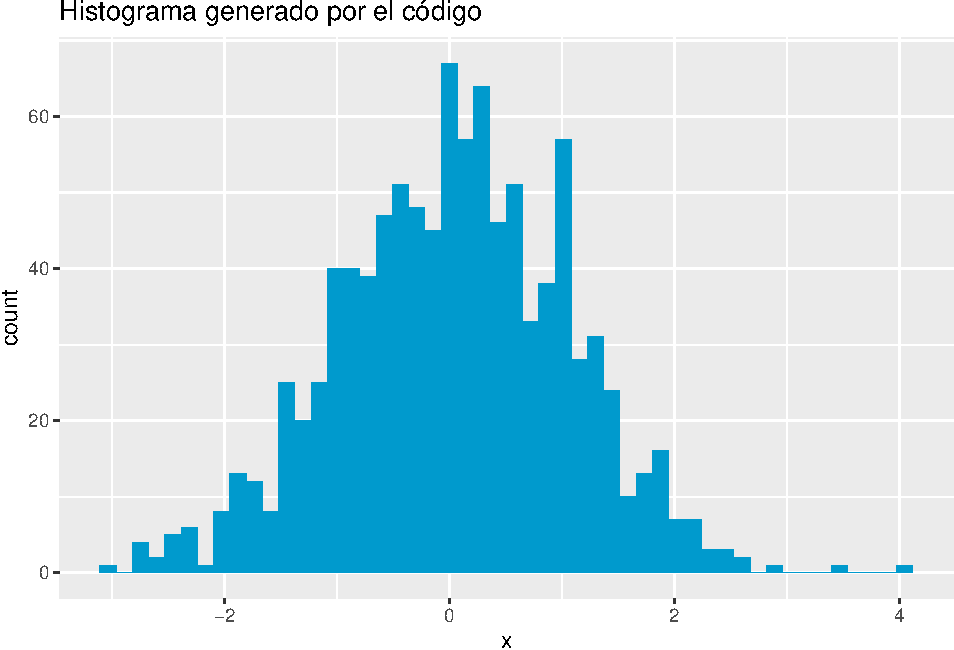
\includegraphics{Introduccion_a_Muestreo_files/figure-latex/unnamed-chunk-81-1} \end{center}

\textbf{NIVEL 3}

\begin{enumerate}
\def\labelenumi{\arabic{enumi}.}
\tightlist
\item
  Instala el paquete \texttt{devtools} (para hacerlo probablemente necesites instalar más cosas en tu computadora; averigua cuáles)
\item
  Usa \texttt{devtools} para instalar el paquete \href{https://github.com/dill/emoGG}{\texttt{emoGG}} desde Github.
\item
  Verifica que tu instalación fue correcta haciendo la siguiente gráfica:
\end{enumerate}

\begin{Shaded}
\begin{Highlighting}[]
\KeywordTok{library}\NormalTok{(emoGG)}
\KeywordTok{ggplot}\NormalTok{(mtcars, }\KeywordTok{aes}\NormalTok{(wt, mpg))}\OperatorTok{+}\StringTok{ }\KeywordTok{geom_emoji}\NormalTok{(}\DataTypeTok{emoji=}\StringTok{"1f697"}\NormalTok{)}
\end{Highlighting}
\end{Shaded}

\begin{center}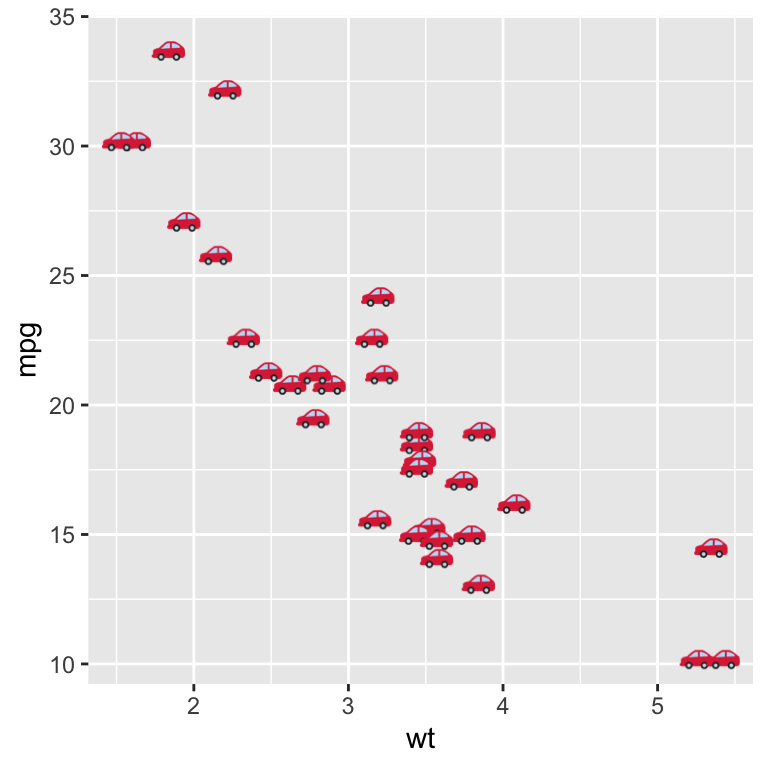
\includegraphics{Introduccion_a_Muestreo_files/figure-latex/unnamed-chunk-82-1} \end{center}

\hypertarget{comentarios-adicionales-sobre-el-formato}{%
\section{Comentarios adicionales sobre el formato}\label{comentarios-adicionales-sobre-el-formato}}

Así como en el español existen reglas de gramática para ponernos todos de acuerdo y entendernos entre todos, en \texttt{R} también existen \emph{sugerencias} a seguir para escribir tu código. Las sugerencias que aquí aparecen fueron adaptadas de las que \href{https://google.github.io/styleguide/Rguide.xml}{utiliza el equipo de \texttt{Google}}.

\begin{enumerate}
\def\labelenumi{\arabic{enumi}.}
\item
  No escribas líneas de más de 80 caracteres (si se salió de tu pantalla, mejor continúa en el siguiente renglón).
\item
  Coloca espacios entre operadores \texttt{+,*,/,-,\textless{}-,=,\ \textless{},\ \textless{}=,\ \textgreater{},\ \textgreater{}=,\ ==} y usa paréntesis para agrupar:
\end{enumerate}

\begin{Shaded}
\begin{Highlighting}[]
\CommentTok{#Esto no se ve muy bien}
\KeywordTok{abs}\NormalTok{(}\DecValTok{3}\OperatorTok{*}\DecValTok{5}\OperatorTok{/}\NormalTok{(}\DecValTok{4-9}\NormalTok{)}\OperatorTok{^}\DecValTok{2-60}\OperatorTok{/}\DecValTok{100-888}\FloatTok{+0.1}\OperatorTok{*}\DecValTok{8888-4}\OperatorTok{/}\DecValTok{10}\OperatorTok{*}\DecValTok{2}\NormalTok{) }\OperatorTok{<}\StringTok{ }\DecValTok{1}\NormalTok{.e}\DecValTok{-6}

\CommentTok{#Los espacios permiten distinguir el orden de las operaciones}
\KeywordTok{abs}\NormalTok{( (}\DecValTok{3} \OperatorTok{*}\StringTok{ }\DecValTok{5}\NormalTok{) }\OperatorTok{/}\StringTok{ }\NormalTok{(}\DecValTok{4} \OperatorTok{-}\StringTok{ }\DecValTok{9}\NormalTok{)}\OperatorTok{^}\DecValTok{2} \OperatorTok{-}\StringTok{ }\DecValTok{60} \OperatorTok{/}\StringTok{ }\DecValTok{100} \OperatorTok{-}\StringTok{ }\DecValTok{888} 
      \OperatorTok{+}\StringTok{ }\NormalTok{(}\FloatTok{0.1} \OperatorTok{*}\StringTok{ }\DecValTok{8888}\NormalTok{) }\OperatorTok{-}\StringTok{ }\NormalTok{(}\DecValTok{4} \OperatorTok{/}\StringTok{ }\DecValTok{10}\NormalTok{) }\OperatorTok{*}\StringTok{ }\DecValTok{2}\NormalTok{ ) }\OperatorTok{<}\StringTok{ }\DecValTok{1}\NormalTok{.e}\DecValTok{-6}
\end{Highlighting}
\end{Shaded}

\begin{enumerate}
\def\labelenumi{\arabic{enumi}.}
\setcounter{enumi}{2}
\tightlist
\item
  Intenta alinear la asignación de variables para legibilidad:
\end{enumerate}

\begin{Shaded}
\begin{Highlighting}[]
\CommentTok{#Esto no tanto}
\NormalTok{altura <-}\StringTok{ }\FloatTok{1.80}
\NormalTok{peso <-}\StringTok{ }\DecValTok{80}
\NormalTok{edad <-}\StringTok{ }\DecValTok{32}

\CommentTok{#Esto se ve bien}
\NormalTok{altura <-}\StringTok{ }\FloatTok{1.80}
\NormalTok{peso   <-}\StringTok{ }\DecValTok{80}
\NormalTok{edad   <-}\StringTok{ }\DecValTok{32}
\end{Highlighting}
\end{Shaded}

\begin{enumerate}
\def\labelenumi{\arabic{enumi}.}
\setcounter{enumi}{3}
\tightlist
\item
  Utiliza nombres que evoquen la variable que representas
\end{enumerate}

\begin{Shaded}
\begin{Highlighting}[]
\CommentTok{#Cuando regreses a esto no sabrás ni qué}
\NormalTok{x <-}\StringTok{ }\DecValTok{10}
\NormalTok{y <-}\StringTok{ }\DecValTok{2}
\NormalTok{z <-}\StringTok{ }\FloatTok{3.14}
\NormalTok{W <-}\StringTok{ }\NormalTok{z }\OperatorTok{*}\StringTok{ }\NormalTok{x}\OperatorTok{^}\NormalTok{y }\CommentTok{#¿Qué calculé?}

\CommentTok{#Es mejor especificar la variable}
\NormalTok{radio        <-}\StringTok{ }\DecValTok{10}
\NormalTok{potencia     <-}\StringTok{ }\DecValTok{2}
\NormalTok{pi_aprox     <-}\StringTok{ }\FloatTok{3.14}
\NormalTok{area_circulo <-}\StringTok{ }\NormalTok{pi_aprox }\OperatorTok{*}\StringTok{ }\NormalTok{radio}\OperatorTok{^}\NormalTok{potencia}
\end{Highlighting}
\end{Shaded}

\begin{enumerate}
\def\labelenumi{\arabic{enumi}.}
\setcounter{enumi}{4}
\tightlist
\item
  No utilices un nombre demasiado similar para cosas diferentes.
\end{enumerate}

\begin{Shaded}
\begin{Highlighting}[]
\CommentTok{#Aquí, seguro eventualmente te vas a equivocar}
\NormalTok{altura <-}\StringTok{ }\DecValTok{10}   \CommentTok{#Altura del edificio}
\NormalTok{Altura <-}\StringTok{ }\FloatTok{1.8}  \CommentTok{#Mi altura}
\NormalTok{ALTURA <-}\StringTok{ }\DecValTok{2000} \CommentTok{#La altitud de la CDMX}

\CommentTok{#Siempre elegir nombres claros, aunque largos}
\NormalTok{altura.edificio <-}\StringTok{ }\DecValTok{10}   \CommentTok{#Altura del edificio}
\NormalTok{altura.Rodrigo  <-}\StringTok{ }\FloatTok{1.8}  \CommentTok{#Mi altura}
\NormalTok{altura.CDMX     <-}\StringTok{ }\DecValTok{2000} \CommentTok{#La altitud de la CDMX}
\end{Highlighting}
\end{Shaded}

\begin{enumerate}
\def\labelenumi{\arabic{enumi}.}
\setcounter{enumi}{5}
\tightlist
\item
  Comenta:
\end{enumerate}

\begin{Shaded}
\begin{Highlighting}[]
\CommentTok{#¿Qué hace esto?}
\NormalTok{x <-}\StringTok{ }\DecValTok{168}
\NormalTok{x <-}\StringTok{ }\NormalTok{x}\OperatorTok{/}\DecValTok{100}
\NormalTok{y <-}\StringTok{ }\FloatTok{71.2}
\KeywordTok{print}\NormalTok{(y}\OperatorTok{/}\NormalTok{x}\OperatorTok{^}\DecValTok{2}\NormalTok{) }
  
\CommentTok{#Es mejor así}
\NormalTok{altura <-}\StringTok{ }\DecValTok{168}        \CommentTok{#en centímetros}
\NormalTok{altura <-}\StringTok{ }\NormalTok{altura}\OperatorTok{/}\DecValTok{100} \CommentTok{#en metros}
\NormalTok{peso   <-}\StringTok{ }\FloatTok{71.2}       \CommentTok{#peso en kg}
\KeywordTok{print}\NormalTok{(peso}\OperatorTok{/}\NormalTok{altura}\OperatorTok{^}\DecValTok{2}\NormalTok{) }\CommentTok{#índice masa corporal}
\end{Highlighting}
\end{Shaded}

\begin{figure}

{\centering 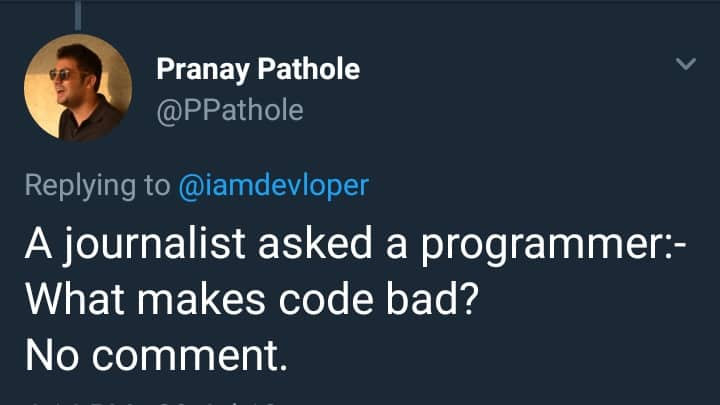
\includegraphics[width=10in]{images/tweet1} 

}

\caption{Trad: Un periodista se acerca a un programador a preguntarle ¿qué hace que un código sea malo? -Sin comentarios.}\label{fig:unnamed-chunk-88}
\end{figure}

\begin{enumerate}
\def\labelenumi{\arabic{enumi}.}
\setcounter{enumi}{6}
\tightlist
\item
  Siempre pon las llamadas a los paquetes y el directorio al inicio de tu archivo para que otro usuario sepa qué necesita.
\end{enumerate}

Código limpio y legible:

\begin{Shaded}
\begin{Highlighting}[]
\CommentTok{#Asumiendo aquí inicia el archivo:}
\KeywordTok{setwd}\NormalTok{(}\StringTok{"Mi directorio"}\NormalTok{)}

\CommentTok{#Llamamos la librería}
\KeywordTok{library}\NormalTok{(beepr)}
\KeywordTok{library}\NormalTok{(tidyverse)}

\CommentTok{#Analizamos una base de datos de R}
\KeywordTok{data}\NormalTok{(iris) }\CommentTok{#Base de datos de flores}

\CommentTok{#Agrupamos la base por especie}
\NormalTok{iris.agrupada <-}\StringTok{ }\KeywordTok{group_by}\NormalTok{(iris, Species)}

\CommentTok{#Obtenemos la media por longitud de sépalo}
\NormalTok{iris.media    <-}\StringTok{ }\KeywordTok{summarise}\NormalTok{(iris.agrupada, }\DataTypeTok{SL.mean =} \KeywordTok{mean}\NormalTok{(Sepal.Length))}

\CommentTok{#Avisa que ya terminó}
\KeywordTok{beep}\NormalTok{(}\DecValTok{5}\NormalTok{)}
\end{Highlighting}
\end{Shaded}

es siempre preferible a código escrito \emph{con prisas} :

\begin{figure}

{\centering 
\includegraphics[width=8.89in]{images/Grandma-Finds-The-Internet} 

}

\caption{Yo, leyendo mi código no comentado y con mala edición 6 meses después de haberlo hecho.}\label{fig:unnamed-chunk-90}
\end{figure}

\begin{Shaded}
\begin{Highlighting}[]
\KeywordTok{data}\NormalTok{(iris);}\KeywordTok{setwd}\NormalTok{(}\StringTok{"Mi directorio"}\NormalTok{)}
\KeywordTok{library}\NormalTok{(tidyverse);x<-}\KeywordTok{group_by}\NormalTok{(iris,Species  )}
\CommentTok{#Aquí hacemos esto}
\NormalTok{iris.means=}\KeywordTok{summarise}\NormalTok{( x,}\DataTypeTok{SL.mean=}\KeywordTok{mean}\NormalTok{(Sepal.Length));}\KeywordTok{library}\NormalTok{(beepr);}\KeywordTok{beep}\NormalTok{(}\DecValTok{5}\NormalTok{)}\CommentTok{#FIN}
\end{Highlighting}
\end{Shaded}

Siempre escribe tu código pensando que alguien más (\href{https://www.redaccionmedica.com/virico/noticias/el-gato-de-schrodinger-y-por-que-no-abrir-la-puerta-cerrada-de-la-consulta-5188}{y ese alguien más puedes ser tú}) va a leerlo. ¡No olvides comentar!

  \bibliography{book.bib,packages.bib}

\end{document}
